\documentclass[12pt,a4paper]{report}     % font size= 12,paper size= a4, document type= report 
\usepackage{graphics}
\usepackage[font=small,labelfont=bf]{caption}
\usepackage{fancybox}		% For formatting of cover page5
\usepackage{amsmath}    	% For  mathematical formulae
\usepackage{amssymb}
\usepackage{setspace}		% For adjusting line spacing 
\usepackage{pdfpages}
\usepackage{hyperref}                     % pacakage for 
\usepackage{fancyhdr}
\usepackage{float}
\usepackage{adjustbox}
% pacakage for including header and footer 
%\usepackage{times}                        % package for font type
\usepackage[left=1in,right=1in,top=1in,bottom=0.8in]{geometry} %
\usepackage{url}
\usepackage{rotating}
\usepackage{array}
\usepackage{enumitem}
%\usepackage{bbding}
\usepackage{amsfonts}

\makeatletter
\def\@makechapterhead#1{%
  \vspace*{5\p@}%
  {\parindent \z@ \raggedright \normalfont
    \ifnum \c@secnumdepth >\m@ne
       \LARGE\bfseries \space \thechapter. \space
    \interlinepenalty\@M
    \LARGE \bfseries #1\par\nobreak
    \vskip 10\p@
  }}
  \makeatother
\begin{document}
\newpage
\pagestyle{plain}
\pagestyle{empty}
\pagestyle{fancy}							%display header, footer
\renewcommand{\headrulewidth}{0pt}
%\pagenumbering{arabic}						%display page numbers in arabic								 %set header to left	

%\fancyfoot[LO]{\textit{P:F-SMR-UG/08/R0}}			%set footer to left
\fancypagestyle{plain}{}

 %\thispagestyle{empty}
	\pagenumbering{gobble}
	\thisfancyput(-0.0in,-10.0in){%
	%\thisfancypage{%
%\setlength{\fboxrule}{1pt}\doublebox}{} 
\setlength{\unitlength}{1in}\framebox(6.7,10.2)}
\begin{center}
      
      \begin{center} {A} \end{center}
      \vspace{0.2 in}
      { FINAL PROJECT REPORT}
      \vspace{0.2 in}\\
       ON
			\end{center}
	\begin{center}
	    \vspace{0.1 in}
		\textbf{\large  Medical Abstract Segmentation  } % Give Your Seminar Title
		\vspace{0.2 in}
	\end{center}
     \vspace{0.2 in}
		\begin{center}
	    SUBMITTED TO THE SAVITRIBAI PHULE PUNE UNIVERSITY, PUNE \\
	    IN PARTIAL FULFILLMENT OF THE REQUIREMENTS\\
	    FOR THE AWARD OF THE DEGREE OF
	\end{center}
	\vspace{0.1 in}
	
	\begin{center}
	   {BACHELOR OF ENGINEERING}\\
	    \begin{small}{ INFORMATION TECHNOLOGY}
\end{small}	\end{center}
	\vspace{0.1 in}
	
	\begin{center}
	   \textbf{BY}
	\end{center}
	\vspace{0.1 in}
	
	\begin{center}
\begin{tabular}{ c c }
    
    Saifuddin Shaikh &  B190058702 \\
    Rishikesh Suryavanshi & B190058720 \\
    Pranish Warke & B190058739 \\
\end{tabular}
 
	\end{center}
	\vspace{0.1 in}
	
	\begin{center}
	    {Under the guidance of }\\
	    {\textbf{Dr. Emmanuel M.}}  % Here write Your Seminar Guide Name
	\end{center}

		\vspace{0.075in}

	\begin{center}
	  \begin{figure}[h]
			\centering
			
\includegraphics[scale=1.5]{pict_logo.png}
		\end{figure}
		\vspace{0.1cm}
	  \begin{large}\textsc {Department Of Information Technology} \end{large}\\
	  \textsc{Pune Institute of Computer Technology}\\
%	  \textsc{Sr. No 27, Near Trimurti Chowk, Dhankawadi}\\
	  \textsc{Pune - 411 043.}\\
	      \textbf{2023-2024}
	\end{center}

%------------------------------------------------------------------------------
%  Cover ends here
%------------------------------------------------------------------------------
%------------------------------------------------------------------------------
%  Certificate starts here
%------------------------------------------------------------------------------
\newpage
\pagestyle{plain}
\pagestyle{empty}
\pagestyle{fancy}							%display header, footer
\renewcommand{\headrulewidth}{0pt}
%\pagenumbering{arabic}						%display page numbers in arabic								 %set header to left	
%\fancyfoot[LO]{\textit{P:F-SMR-UG/08/R0}}			%set footer to left
\fancypagestyle{plain}{}

 %\thispagestyle{empty}
		\pagenumbering{roman}
		
	\thisfancyput(-0.15in,-9.7in){%
	%\thisfancypage{%
%\setlength{\fboxrule}{1pt}\doublebox}{} 
\setlength{\unitlength}{1in}\framebox(6.7,10.2)}
\begin{center}

{ SCTR's
   PUNE INSTITUTE OF COMPUTER TECHNOLOGY \\
   \small{DEPARTMENT OF INFORMATION TECHNOLOGY} \\

}
\vspace{0.10in}

\vspace{0.1in}

\includegraphics[scale=1.5]{pict_logo.png}
\end{center}
\vspace{0.075in}
\begin{center}
\textbf{\underline{C E R T I F I C A T E}}
\vspace{0.08in}
\end{center}
		\noindent
  				\setlength{\baselineskip}{1.1\baselineskip}
	\begin{center}
This is to certify that the final project report entitled  \\
		\textbf{Medical Abstract Segmentation} 
\singlespace
submitted by\\
\begin{center}
\begin{tabular}{ c c }
    Saifuddin Shaikh & B190058702 \\
    Rishikesh Suryavanshi & B190058720 \\
    Pranish Warke & B190058739 \\
\end{tabular}
 
	\end{center}
	\end{center}

\onehalfspace
\begin{quote}
is a bonafide work carried out by them under the supervision and guidance of \textbf{Dr.Emmanuel M.} and
it is approved for the partial fulfillment of the requirement of Savitribai Phule Pune University for the award of the Degree of Bachelor of Engineering (Information Technology).\\

This project report has not been earlier submitted to any other Institute or University for the award of any degree or diploma.\\
\end{quote}
		\noindent 
		


\begin{quote}
\singlespace
%\\[0.5in]
\textbf{Dr. Emmanuel M.} % include Seminar Guide Name
\hspace{2in} \textbf{Dr. A. S. Ghotkar}\\
Project Guide\hspace{3.2 in}       HOD IT \\\\\\

\textbf{} % include Seminar Guide Name
\hspace{3.7in} \textbf{Dr. S. T. Gandhe}\\
SPPU External Guide\hspace{2.7in}       Principal \\\\\\

Date:       \\ %write date in the form of dd/mm/yyyy format
Place:       %write place as Pune
\\\\


 \end{quote}
\addcontentsline{toc}{section}{Certificate}
%------------------------------------------------------------------------------
%  Certificate ends here
%------------------------------------------------------------------------------

\newpage	
\pagestyle{plain}
%\pagestyle{empty}
\pagestyle{fancy}							%display header, footer
\renewcommand{\headrulewidth}{0pt}
%\pagenumbering{arabic}						%display page numbers in arabic								 %set header to left	
\fancyfoot[LO]{\textit{}}			%set footer to left
\fancypagestyle{plain}{}%start a new page
		\pagestyle{plain}           %dont display header footer and page nos
%\vline
		\begin{center}				%centre align the text
			\begin{LARGE}
	\section*{Acknowledgement}
			\addcontentsline{toc}{section}{Acknowledgement}
				%leave space of 0.5 inches vertically
			\end{LARGE}
		\end{center}
		\begin{normalsize}
%				\begin{quote}
{\setlength{\baselineskip}{1.1\baselineskip}
\noindent %Start acknowledgement from here.
With deep sense of gratitude we would like to thanks all the people who have lit our path with their
kind guidance for our Project Selection, Design and Development. We are very grateful to these
intellectuals, experts, who did their best to help during our completion of project work.
\newline
It is our proud privilege to express deep sense of gratitude to the Principal, Prof. S. T. Gandhe,
SCTR's Pune Institue of Computer Technology, Pune for his comments and kind permission to complete this project. We
remain indebted to Prof. Archana S. Ghotkar, Head of Informattion Technology Department for her timely
suggestion and valuable guidance.
\newline
The special gratitude goes to our Internal Project Guide Dr. Emmanuel Markappa, staff members,
technical staff members of Information Technology Department for his/her technical, timely, excellent
and coercive guidance in completion of this project work. We thanks to all the class colleagues for
their appreciable, encouraging help for completion of our project.








			\vspace{1.8in}
				\begin{flushright} 
\begin{tabular}{ c c }
    
   Saifuddin Shaikh & B190058702 \\
    Rishikesh Suryavanshi & B190058720 \\
    Pranish Warke & B190058739 \\
\end{tabular}
 \end{flushright}
%				\end{quote}

}
		\end{normalsize}
		

\newpage
%-----------------------------------Abstract------------------------------------------
		\newpage					%start a new page
		\pagestyle{plain}           %dont display header footer and display page nos
		\begin{center}				%centre align the text
			\begin{LARGE}
						\section*{ Abstract}
			%\vspace{.15 in}       %leave space of 0.5 inches vertically
			\end{LARGE}
		\end{center}
		\begin{normalsize}
{\setlength{\baselineskip}{1.1\baselineskip}   %set line spacing as 1.5
\noindent % Start writing abstract from here.
Randomized control trials (RCTs) are essential for evaluating the effectiveness of medical interventions, but their results are often buried within lengthy and complex documents. Efficiently extracting and organizing critical information from RCT abstracts can significantly impact evidence-based decision-making and healthcare research. The automated segmentation of medical abstracts is a vital component of medical information retrieval and analysis, significantly impacting clinical decision-making, healthcare research, and knowledge discovery. This paper presents an innovative approach to segmenting abstracts of RCTs through the application of natural language processing (NLP) and neural networks. The practical applications of NLP and neural network-based text segmentation in the context of RCTs are exemplified, ranging from systematic reviews and meta-analyses to the development of clinical guidelines. Case studies are presented to showcase the impact of this technology in improving the accessibility and utilization of RCT results. This paper serves as a valuable resource for researchers, healthcare professionals, and data scientists, offering a glimpse into the future of RCT abstract segmentation. It underscores the pivotal role of NLP and neural networks in unlocking the potential of RCT data, ultimately advancing the field of evidence-based medicine and healthcare decision-making.\\\\ 
\textbf{Keywords:} % start writing Keywords from here
medical abstract,text segmentation,randomized control trial (RCT),natural language processing(NLP),neural networks\\\\
\par}
		\end{normalsize}
\addcontentsline{toc}{section}{Abstract}
%---------------------------------Abstract ends---------------------------------------
\newpage

\thispagestyle{empty}
\fancyhead{}
\renewcommand{\headrulewidth}{0pt}
%\fancypagestyle{plain}{}%start a new page
%		\thispagestyle{plain} 

\addcontentsline{toc}{section}{Contents}
\tableofcontents	 								% auto generate table of contents
\newpage
{\setlength{\baselineskip}{1.1\baselineskip}        % auto generate list of figures  
\listoffigures
\addcontentsline{toc}{section}{List of Figures}   % add to table of contents
}
\newpage
{\setlength{\baselineskip}{1.1\baselineskip}        % auto generate list of tables   
\listoftables
\addcontentsline{toc}{section}{List of Tables}
}
%---------------------------Abbrevations------------------------------------------------------------
\newpage
		\begin{LARGE}
			\begin{flushleft}
				\section*{\centering{Abbreviations}}
			\end{flushleft}
		\end{LARGE}
		\addcontentsline{toc}{section}{Abbreviations}	
\begin{normalsize}
					\noindent
{\setlength{\baselineskip}{1.1\baselineskip}
\vspace{0.2 in}
\begin{tabular}{lll}
\vspace{0.1 in}
LSTM	&	:	&	Long Short Term Memory	\\
\vspace{0.1 in}
BERT	&	:	&	Bidirectional Encoder Representations from Transformers\\
\vspace{0.1 in}
RCT	&	:	&	Randomised Control Trial 	\\
\vspace{0.1 in}
NLP	&	:	&	Natural Language Processing 	\\
\vspace{0.1 in}
GRU	&	:	&	Gated Recurrent Unit 	\\
\end{tabular}
\par}
\end{normalsize}

%-----------------------------------Chapter 1 Introduction}
\newpage
%\clearpage
\pagestyle{fancy}							%display header, footer
\pagenumbering{arabic}	%display page numbers in arabic
\renewcommand{\headrulewidth}{0.5pt}
\fancyhead[RO]{\textit{Project Title }} %set header to right
\fancyhead[LO]	{}											 %set header to left	
\renewcommand{\footrulewidth}{0.5pt}		% print horizontal line in the footer of 0.5 pt
\fancyfoot[RO]{\textit{Dept. of Information Technology}}		%set footer to right
\fancyfoot[LO]{\textit{PICT,Pune}}			%set footer to left
\fancypagestyle{plain}{}
\pagenumbering{arabic}	
\chapter{\centering{Introduction}}
\begin{normalsize}
			\noindent

%-------------------------------------------------------------------------------------------------------
%  Start writing from here.
%(short para about your area describing its place in the world of Technology)
\section{Introduction} 	
{\setlength{\baselineskip}{1.1\baselineskip}
%Start writing from here.
Randomized Controlled Trial (RCT) is a specific type of study design commonly used in medical research to evaluate the effectiveness of a treatment or intervention. In an RCT, participants are randomly assigned to different groups to compare the outcomes of those who receive the treatment or intervention with those who do not. Existing models based on artificial neural networks (ANNs) for sentence classification often do not incorporate the context in which sentences appear and classify sentences individually.
The scope of medical abstract segmentation for RCTs using NLP and neural networks encompasses a wide range of applications that contribute to the advancement of healthcare, medical research, and clinical decision-making. This field con- tinues to evolve, driven by the increasing volume of medical literature and the need for more efficient ways to extract valuable insights from this vast body of knowledge.
For a variety of Natural Language Processing (NLP) activities, such as information retrieval, information extraction, and text summarization, structuring the unstructured Randomized Controlled Trial (RCT) is helpful. One example is classifying sentences into Background, Objective, Methods, Results, and Conclusion. However, a large number of PubMed abstracts lack hierarchical organization. Only about 30\% of all PubMed abstracts, according to Ripple et al. (2014), include their structural information, which hinders effective knowledge discovery and information retrieval from those sizable biomedical bibliographic databases. Sentence classification for medical abstracts has been the subject of a lot of studies.
The aim of "Medical Abstract Segmentation" is to focus on classifying sentences in medical abstracts, and particularly in randomized controlled trials (RCTs), as they are commonly considered to be the best source of medical evidence. 
\par
}	
\section{Motivation}
{\setlength{\baselineskip}{1.1\baselineskip}
%Start writing from here.
With the unprecedented growth of biomedical publications, structured abstracts in bibliographic databases  like PubMed are essential for assisting researchers with information retrieval and knowledge synthesis.
The number of Biomedical articles continue to grow. As of February 25th, 2022, PubMed a popular bibliographic database that aids scholars in locating articles of interest has over 40,000,000 publicly accessible abstracts. Medical abstracts structural information, such as the Background, Objective, Methods, Results, and Conclusion subsections, is helpful for a variety of Natural Language Processing (NLP) applications, including text summarization, information extraction, and information retrieval. However, a large number of PubMed abstracts lack subsection organization. Franck notes that more than half of all PubMed abstracts include their structural information [1], which restricts the amount of material that can be efficiently retrieved and knowledge that can be discovered from those extensive biomedical bibliographic databases. Thus, it is beneficial to create automated techniques for categorizing statements in biomedical abstracts into different subsections.
\par}	

\section{Objectives}
{\setlength{\baselineskip}{1.1\baselineskip}
%Start writing from here.
To enable more precise and relevant retrieval of medical information from abstracts by breaking them down into smaller, semantically coherent segments.
To facilitate the extraction of critical information from abstracts, including study objectives, methods, results, and conclusions. 
To assist healthcare professionals in making informed clinical decisions by providing them with easily accessible and relevant information from medical abstracts.
}
\section {Scope}
{\setlength{\baselineskip}{1.1\baselineskip}
%Start writing from here.
The scope of medical abstract segmentation of Randomized Controlled Trials (RCTs) using Natural Language Processing (NLP) is substantial and holds great promise in the realm of healthcare and medical research. NLP-powered abstract segmentation offers the potential to transform the way we access and utilize critical information from RCTs. By breaking down RCT abstracts into structured sections and applying NLP techniques, we can enhance information retrieval, facilitate systematic literature reviews, automate data extraction for meta-analyses, and categorize content for more efficient referencing. Moreover, NLP enables semantic analysis and knowledge discovery, promoting evidence-based medicine by automating the identification of relevant clinical information. This structured data can also integrate seamlessly into clinical decision support systems, offering real-time insights for healthcare providers. With the continual evolution of NLP, the scope of medical abstract segmentation will only expand, making this technology an invaluable asset in the pursuit of improved healthcare practices and medical research.
}


%-----------------------Literature Survey & Discussion (Literature Survey)----------------
\newpage 
\chapter{\centering{Literature Survey}}
{\setlength{\baselineskip}{1.1\baselineskip}
%Start writing from here.
\section{Existing Methodologies}
In many branches of natural language processing, including sentiment analysis, question answering, and dialog management, short-text classification is a crucial problem.A comprehensive study has been done on text classification in the domain of medical research papers. Some of the most recent and prominent ones have been used for this literature survey. 

In [1] the dataset consists of approximately 200,000 abstracts of randomized controlled trials, totaling 2.3 million sentences. Each sentence of each abstract is labeled with its role in the abstract using one of the following classes: background, objective, method, result, or conclusion, and PubMed 200k RCT is a substantial dataset designed for sequential sentence classification, is introduced. It notably stands as one of the largest datasets of its kind known to date. The evaluation encompasses the performance assessment of various baseline models, providing a valuable reference for researchers to readily benchmark their algorithms without the necessity of creating their own foundational benchmarks.

[2] suggests a novel uniform deep learning architecture and multi-task learning approach for cross-domain sequential sentence classification in scientific texts. This paper introduces a comprehensive deep-learning architecture designed for sequential sentence classification, demonstrating remarkable advancements, particularly in full paper datasets, without the need for intricate feature engineering. The authors conduct a thorough investigation and comparison of transfer learning approaches, shedding light on the exceptional effectiveness of multi-task models applied across diverse datasets. Furthermore, this study places significant emphasis on the crucial notion of semantic relatedness between classes within varying dataset annotation schemes. It proposes a practical and robust method for identifying and establishing these semantic connections. Such an approach bears the promise of unlocking the potential for cross-discipline applications in the domain of sentence classification, with particular relevance to academic search engines and information retrieval systems.

Similarly [3] Adopted a deep learning neural network model and pretrained the network on PubMed non-RCT dataset. Transfer Learning with fine-tuning was done on the hand-labeled dataset they created from scratch. The PubMed-non-RCT corpus was converted into a three-class dataset, and their model was trained on it. They achieved 92.1\% accuracy on the PubMed-non-RCT dataset. The model was then evaluated on various CS corpora using different approaches: 'Locally-trained,' 'Pre-trained on PubMed,' and 'Fine-tuned'. Notably, 'Fine-tuned' transfer learning significantly improved the model, while 'Pre-trained on PubMed' performed worse than local training, indicating the dissimilarity between the CS and biomedical corpora. Despite such differences, transfer learning with fine-tuning still provided more than a 10\% accuracy boost, even with entirely dissimilar datasets. The paper introduces a method for automatic discourse classification in computer science abstracts, showing that transfer learning with fine-tuning yields impressive results, even with limited labeled data. The model effectively generalizes across CS sub-fields, despite variations in discourse classification due to presentation style differences.

In [4] The model is composed of four components: the word embedding layer, the sentence encoding layer, the context enriching layer, and the label sequence optimization layer. The sequence of embedding vectors is first processed by a bi-directional RNN (bi-RNN) or CNN layer. In this work, they introduced an ANN-based hierarchical sequential labeling network designed to classify sequentially appearing sentences in text. By incorporating contextual information from neighboring sentences through an LSTM layer, they observed a significant enhancement in prediction quality. Their model demonstrated a notable 2\%-3\% improvement over state-of-the-art results in two datasets focusing on sequential sentence classification within medical abstracts. This proposed model's potential for generalization to various problems related to sequential sentence classification, including paragraph-level sequential sentence categorization in full-text articles, presents promising opportunities for text mining and document retrieval.

In [5] The model consists of two novel components: supervised local attention and an auxiliary span-based classification task. The proposed model aims to capture the latent segment structure of the document by considering the coherent semantics of contiguous sentences. It utilizes dynamic local attention to explicitly capture the structural information. 

In [6] a Machine Learning approach that aims to classify sentences according to the PIBOSO scheme is presented. A discriminative set of features that do not rely on any external resources to achieve results is used. In this paper, they introduced a machine-learning approach for identifying scientific artifacts in biomedical abstracts within the context of Evidence-Based Medicine. Their approach utilized sentence classification following the PIBOSO scheme. Importantly, their approach did not rely on external resources for classification features. The results demonstrated a significant improvement over existing methods, achieving a micro-average F-score of 90.74\% and 87.21\% for structured and unstructured abstracts, respectively. This marks a substantial increase compared to prior approaches.

In [7] The algorithm implemented is based on the following four steps:  Medical concepts are extracted from free-text descriptions of an interview and examination, a new representation of identified concepts is derived using concept embedding, concept embeddings are transformed into visit embeddings and clustering is performed on visit embeddings. They used two of the most common: k-means and hierarchical clustering with Ward’s method for merging clusters.  These algorithms cover two different clustering approaches. The algorithms are memory and time-efficient, so no need to use more advanced methods. 

[8] and [9] propose a few-shot prompt learning-based approach to classify sentences in medical abstracts of randomized clinical trials (RCT) and observational studies (OS) to subsections of Introduction, Background, Methods, Results, and Conclusion. 5 manually designed templates in a combination of 4 BERT model variants were tested and compared to a previous Hierarchical Sequential Labeling Network architecture and traditional BERT-based sentence classification method. Four deep learning models, namely RNN, LSTM, GRU, and BLSTM are used. Data pre-processing steps are applied that include: text cleaning, tokenization, stemming, as well as lemmatization to remove and stop words. Their approach achieves state-of-the-art results on all three datasets, surpassing Jin and Szolovits (2018) and their BERT-based baselines. The performance gap between their baselines and their best model is more pronounced for smaller datasets (CSABSTRUCT, NICTA) and narrower for the larger dataset (PUBMED-RCT), underlining the significance of pretraining for smaller datasets. To delve into the advantages of their joint sentence encoding relative to the BERT+Transformer baseline, they qualitatively analyze examples from CSABSTRUCT. They discover that a significant portion of such examples require contextual information for accurate classification, emphasizing the need for context in certain instances. In [10] ULMFiT stands as a game-changer in NLP, it delivers remarkable error reductions of 18-24 percent across six text classification tasks. Its open-sourced pre-trained models and code empower the NLP community with powerful tools for diverse applications.
[10] discusses the impact of inductive transfer learning on computer vision (CV) and how it has influenced deep neural networks in CV. It mentions that features in deep neural networks transition from general to task-specific from the first to the last layer, and most work in CV focuses on transferring the first layers of the model .

\begin{table*}%h
\begin{adjustbox}{width=\textwidth, totalheight=\textheight, keepaspectratio}
\begin{tabular}{|p{6cm}|p{8cm}|p{8cm}|p{3cm}|}
\hline
Title &
  Methodologies &
  Inferences &
  Dataset \\ \hline
\begin{tabular}[c]{@{}l@{}}PubMed 200k RCT: a Dataset for \\ Sequential Sentence \\ Classification in Medical Abstracts\end{tabular} &
  \begin{tabular}[c]{@{}l@{}}Dataset is constructed upon MED-\\ LINE/PubMed Baseline Database. \\ Abstracts are selected based on the\\ two criteria: \\ i. It must be an RCT\\ ii. It must be structured\end{tabular} &
  \begin{tabular}[c]{@{}l@{}}• It is the largest such dataset \\    in the field of Medical \\    Research.\\ • It evaluated the performance on \\   several baseline models \\   based on this dataset.\\ • It achieved state of the art results \\   for Bi-ANN model with \\   F1 score of 91.6\end{tabular} &
  \begin{tabular}[c]{@{}l@{}}PubMed \\ 200k RCT\end{tabular} \\ \hline
\begin{tabular}[c]{@{}l@{}}Cross-Domain Multi-Task \\ Learning for Sequential Sentence \\ Classification in Research Papers\end{tabular} &
  \begin{tabular}[c]{@{}l@{}}1. Proposed SciBERT-HSLN architecture.\\ 2. Utilized SciBERT for Word Embeddings.\\ 3. Two approaches are suggested here one \\ without Transfer Learning and one with \\     Transfer Learning.\end{tabular} &
  \begin{tabular}[c]{@{}l@{}}• It achieved state of the art results for \\    PMD dataset with F1 score of 93.1\\ • F1 score of 86.8 for NIC dataset\end{tabular} &
  \begin{tabular}[c]{@{}l@{}}PMD, NIC, \\ ART, DRI\end{tabular} \\ \hline
\begin{tabular}[c]{@{}l@{}}Segmenting Scientific Abstracts \\ into Discourse Categories: \\ A Deep Learning-Based Approach \\ for Sparse Labeled Data\end{tabular} &
  \begin{tabular}[c]{@{}l@{}} Transfer Learning with Fine Tuning was \\ done on the hand labelled dataset \\ they created from scratch.\end{tabular} &
  \begin{tabular}[c]{@{}l@{}}• It was able to achieve 75\% accuracy \\    with the classification of CS abstracts.\end{tabular} &
  \begin{tabular}[c]{@{}l@{}}Hand Labelled \\ corpus of \\ structured \\ CS abstracts\end{tabular} \\ \hline
\begin{tabular}[c]{@{}l@{}}Hierarchical Neural Networks \\ for Sequential Sentence \\ Classification in Medical \\ Scientific Abstracts\end{tabular} &
  \begin{tabular}[c]{@{}l@{}} Model is composed of four layers :\\     i.   Word Embedding layer\\     ii.  Sentence Encoding layer\\     iii. Context Enriching layer\\     iv.  Label Sequence Optimisation layer\end{tabular} &
  • F1 score for PubMed 20k dataset is 92.6 &
  PubMed 20k RCT \\ \hline
\begin{tabular}[c]{@{}l@{}}A Span-based Dynamic\\  Local Attention Model for \\ Sequential Sentence \\ Classification\end{tabular} &
  \begin{tabular}[c]{@{}l@{}} Model consists of two novel components:\\       i. supervised local attention\\       ii. auxiliary span based classification\end{tabular} &
  \begin{tabular}[c]{@{}l@{}}• F1 score of 92.8 on PubMed 20k RCT \\ • F1 score of 86.8 on NICTA-PIBOSO\end{tabular} &
  PubMed 20k RCT \\ \hline
\begin{tabular}[c]{@{}l@{}}Identifying scientific artefacts \\ in biomedical literature: \\ the Evidence Based Medicine \\ use case\end{tabular} &
  \begin{tabular}[c]{@{}l@{}}A machine learning approach that aims \\     to classify sentences according to\\     PIBOSO scheme is presented.\end{tabular} &
  \begin{tabular}[c]{@{}l@{}}• CRF classifier achieves F1 score of 90.74 \\    and 87.21 respectively over structured \\    and unstructured abstracts.\end{tabular} &
  NICTA-PIBOSO \\ \hline
\begin{tabular}[c]{@{}l@{}}Towards More Generalizable and \\ Accurate Sentence \\ Classification in \\ Medical Abstracts with Less Data\end{tabular} &
  \begin{tabular}[c]{@{}l@{}} Few shot prompt based learning approach to \\ classify sentences in medical \\ abstracts was discussed.\end{tabular} &
  \begin{tabular}[c]{@{}l@{}}• The study showed that the HSLN model \\    required only 20\% of the training data to \\    achieve comparable F1 scores when \\    compared with the baseline model.\end{tabular} &
  \begin{tabular}[c]{@{}l@{}}PubMed 200/20k\\ PubMed 20k OS\end{tabular} \\ \hline
\begin{tabular}[c]{@{}l@{}}Interpretable segmentation \\ of medical free-text records \\ based on word\end{tabular} &
  \begin{tabular}[c]{@{}l@{}} K-Means and Hierarchical Clustering with \\ Ward's method was used.\end{tabular} &
  \begin{tabular}[c]{@{}l@{}}• The embeddings outperformed \\    Pennington \\    et al on medical term analogies despite a \\    smaller corpus size.\\ • Future work should explore the dynamic \\    relationship with identified clusters.\end{tabular} &
  \begin{tabular}[c]{@{}l@{}}The Polish corpus \\ of free text \\ clinical records\end{tabular} \\ \hline
\begin{tabular}[c]{@{}l@{}}Pretrained Language Models\\  for Sequential Sentence\\ Classification\end{tabular} &
  \begin{tabular}[c]{@{}l@{}} Four Deep Learning Models\\ namely RNN, LSTM,\\     GRU and BLSTM are used.\end{tabular} &
  \begin{tabular}[c]{@{}l@{}}• Accuracy: BLSTM gives the highest \\    accuracy of 82.18\%\end{tabular} &
  \begin{tabular}[c]{@{}l@{}}Kaggle Dataset \\ having insult \\ labelled \\ comments \\ was used.\end{tabular} \\ \hline
\begin{tabular}[c]{@{}l@{}}Deep Learning Based \\Text Classification: \\ A Comprehensive Review\end{tabular} &
  \begin{tabular}[c]{@{}l@{}} Survey of more than 150 DL models \\was carried,which are developed \\in the past six years and \\ have significantly improved \\     state of the art on various TC tasks\end{tabular} &
  \begin{tabular}[c]{@{}l@{}}• Several state of the art models were used\\    in this paper\end{tabular} &
  \begin{tabular}[c]{@{}l@{}}SQuAD,\\ WikiQA,\\ DBpedia\end{tabular} \\ \hline
\begin{tabular}[c]{@{}l@{}}Universal Language Model Fine-\\ tuning for Text Classification.\end{tabular} &
  \begin{tabular}[c]{@{}l@{}}\\  Proposed discriminative fine-tuning, slanted \\     triangular learning rates, and \\gradual unfreezing\end{tabular} &
  \begin{tabular}[c]{@{}l@{}}• Method suggested significantly \\    outperforms \\    the state-of-the-art  on six text \\    classification tasks, reducing the error  \\    by 18-24\% on the majority \\    of datasets.\end{tabular} &
  \begin{tabular}[c]{@{}l@{}}TREC-6\\ IMDb\\ Yelp-bi Yelp-full\\ DBpedia\\ AG\end{tabular} \\ \hline
\begin{tabular}[c]{@{}l@{}}A Hierarchical Model with \\ Recurrent Convolutional \\ Neural Networks for \\ Sequential Sentence Classification\end{tabular} &
  \begin{tabular}[c]{@{}l@{}} A new approach called SR-RCNN to generate \\     sentence encoding which uses both Bi-RNN \\     and text CNN to capture contextual and \\ literal relevance information\end{tabular} &
  \begin{tabular}[c]{@{}l@{}}• The model performs best on all datasets, \\    promoting previous best published \\    results by 0.5\%, 0.5\%and 2.5\% \\    on the PubMed 20k, PubMed 200k \\    and NICTA-PIBOSO dataset\end{tabular} &
  \begin{tabular}[c]{@{}l@{}}PubMed RCT,\\ NICTA-PIBOSO\end{tabular} \\ \hline
\begin{tabular}[c]{@{}l@{}}Sectioning of Biomedical \\Abstracts: \\ A Sequence of Sequence\\ Classification Task.\end{tabular} &
  \begin{tabular}[c]{@{}l@{}}1. It uses BIOBERT based model, with a \\ moving window to contextualise \\ the abstracts.\\ 2. Proposed SSN-4 Model consisting of \\ following four layers:\\          i. word embedding layer\\          ii. sentence representation layer\\          iii. BLSTM layer\\          iv. CRF layer\end{tabular} &
  \begin{tabular}[c]{@{}l@{}}• The model trained with the MDS \\    performs fairly well in \\    both MDS and RCT data sets\end{tabular} &
  \begin{tabular}[c]{@{}l@{}}A new data set \\ called MDS \\ that is \\ considerably \\ bigger than \\ PubMed RCT\end{tabular} \\ \hline
\end{tabular}
\end{adjustbox}
\caption{Literature Survey}
\end{table*}
\section{Research Gap Analysis}
We came across important research gaps that require special attention in our quest to create a model for sequential sentence classification. Among these gaps, one major finding was that deep learning has not yet been fully exploited for sequential sentence classification on full papers,which shows that for texts consisting of thousands of lines the classification remains difficult. Also structured abstracts in other domains such as computer science papers are uncommon and availability of labelled dataset are also sparse, this hinders the progress of the ongoing research for cross-domain sequential sentence classification.\par

Most existing models focus on classifying sentences into broad categories, such as methods, results, and conclusions. However, in the context of evidence-based medicine, fine-grained classification is essential. Subdividing categories into more specific labels (e.g., participant characteristics, interventions, primary outcomes) can enhance the utility of the models in clinical research.
Furthermore, RCT abstracts are published in multiple languages, and incorporating linguistic diversity is a pressing research gap.
To bridge the gap between research and practical applications, further investigation is required on how sequential sentence classification can be integrated into clinical decision support systems.
\par



}

%---------------------------Analysis & Discussion----------------
\newpage 
\chapter{\centering{Requirement Specification and Analysis}}
{\setlength{\baselineskip}{1.1\baselineskip}
%Start writing from here.
\section{Problem Definition}
Implementing text segmentation techniques using Natural Language Processing on randomised control trial (RCT) abstracts.
\section{Scope}
The scope of sequential sentence classification in RCT medical abstracts is broad and pivotal in the domain of evidence-based medicine. It encompasses the development and application of natural language processing (NLP) techniques to automatically parse and categorize the textual content within these abstracts. This includes recognizing essential elements such as study objectives, methodology, patient populations, interventions, and outcomes. The scope also extends to the integration of machine learning models and the creation of specialized algorithms to enhance the precision and recall of classification. Ultimately, this approach has the potential to revolutionize the systematic review process, enabling faster and more accurate retrieval of pertinent information for healthcare practitioners, researchers, and policymakers, thereby fostering advancements in medical research and patient care.
\section{Objectives}
The primary objectives for sequential sentence classification in randomized controlled trial (RCT) medical abstracts are twofold: Firstly, to identify and categorize the key information contained within these abstracts, such as the study design, intervention, outcomes, and results. This enables healthcare professionals, researchers, and decision-makers to efficiently assess the relevance and significance of the trial. Secondly, this classification aids in data extraction and indexing, contributing to the development of systematic reviews and evidence-based medicine. By accurately classifying and structuring the information in RCT abstracts, the goal is to enhance information retrieval and facilitate evidence synthesis, ultimately improving healthcare decision-making and research in the medical field.
\section{Proposed Methodology}
\subsection{Type of classification}
Sentence classification is a common task in natural language processing (NLP) and can be categorized into various types, depending on the specific problem or goal. Here are some common types of sentence classification:

1.Text Classification: 
    \begin{itemize}[left=2cm]
        \item Sentiment Analysis
        \item Sequential Sentence Classification
        \item Topic Classification
    \end{itemize}

2.Language Understanding:
    \begin{itemize}[left=2cm]
        \item Named Entity Recognition
        \item Part-of-Speech (POS) Tagging
    \end{itemize}
    
3.Document Summarization:
    \begin{itemize}[left=2cm]
        \item Sentence Importance Ranking:
    \end{itemize}

4.Question Answering:
    \begin{itemize}[left=2cm]
        \item Question Type Classification
        \item Answer Type Classification
    \end{itemize}
\subsection{Data import and cleaning}
The dataset was cloned from the publicly available github repository of [1]. The cloned PubMed RCT dataset consisted of four different sub-datasets within it.The four datasets are as follows :

1.PubMed\textunderscore200K\textunderscore RCT

2.PubMed\textunderscore200K\textunderscore RCT\textunderscore numbers\textunderscore replaced\textunderscore with\textunderscore at\textunderscore sign

3.PubMed\textunderscore20K\textunderscore RCT

4.PubMed\textunderscore20K\textunderscore RCT\textunderscore numbers\textunderscore replaced\textunderscore with\textunderscore at\textunderscore sign

Reading the lines from the training text file results in a list of strings containing different abstract samples, the sentences in a sample along with the role the sentence plays in the abstract.

The role of each sentence is prefixed at the start of each line separated by a tab (\textbackslash t) and each sentence finishes with a new line (\textbackslash n).

Different abstracts are separated by abstract ID's (lines beginning with \#\#\#) and newlines (\textbackslash n).

Prior to feature extraction, pre-processing is applied to the text to clean it and retain only the terms that provide valuable information for sentence classification. The cleaning function performs the following actions on the corpus:

1. Converting the text to lowercase.

2. Removal of Stopwords.

3. Stemming and Lemmatization. 

4. Tokenisation

After these steps, the dataset will be ready for feature engineering. 
After these steps, the dataset will be ready for feature engineering. 
\subsection{Feature Engineering}
The data should be transformed into a format that the
model can comprehend after being cleaned and preprocessed.
Feature engineering is a crucial step in the process of sequential sentence classification, a task commonly encountered in natural language processing (NLP) and text analysis. Sequential sentence classification involves assigning one or more labels to each sentence in a sequence, such as in sentiment analysis, named entity recognition, or text categorization. Effective feature engineering can significantly improve the performance of machine learning models used for this purpose.
There are various key aspects of Feature Engineering in Sequential Sentence Classification : 
\begin{enumerate}
    \item Text Representation
    \item Preprocessing
    \item Tokenization
    \item Feature Extraction
    \item Sequence Encoding
    \item Domain-Specific Knowledge
    \item Model Selection
\end{enumerate}

\break
\break
The major drawback of the two previous feature extraction techniques is the loss of the
relationship between words and, as a consequence, the context of a document. To overcome this problem,  a third extraction technique[10]
Word Embedding: The idea is to assign to similar terms close vectors of a continuous
and multidimensional vector space in a way that makes it possible to calculate similarities
between words or sentences thanks to the distance between vectors, as well as to
generalise a sentence into similar sentences, since the vectors will be similar[10].
Now another problem with this is about the context. If the same word is used for different context the word embedding fail to caputre this. 
This is overcomed by BERT which provides contextualized feature vectors.
We are planning to use the PubMedBERT which is a pretrained model on medical abstracts and literature.This model achieves state-of-the-art performance on several biomedical NLP tasks, as shown on the Biomedical Language Understanding and Reasoning Benchmark.
\\
\newpage
\section{Project Requirements}

\subsection{Datasets}
The PubMed 20K RCT dataset was used in this study. The dataset is available at https://github.com/Franck- Dernoncourt/pubmed-rct.
The collection includes 2.3 million phrases from almost 200,000 abstracts of randomized controlled trials. Each abstract's sentences are assigned a class based on their role in the abstract, such as background, objective, method, result, or conclusion.


For the specified problem of medical abstract segmentation, PubMed dataset is publicly available. It consists of following five labels and the number of samples are as follows:

1. METHODS          59353

2. RESULTS          57953

3. CONCLUSIONS      27168

4. BACKGROUND       21727

5. OBJECTIVE        13839
\subsection{Functional Requirements}
\begin{itemize}
    \item Text Extraction
    \item Preprocessing
    \item Sentence Segmentation 
    \item Contextual Understanding
    \item Visualization and Presentation
\end{itemize}
\subsection{Non Functional Requirements}
\begin{itemize}
    \item \textbf{Performance} : Abstracts should be processed by the system rapidly and effectively, especially when handling big text volumes.
    \item \textbf{Accuracy} : Segmentation should be accurate, with minimal errors in identifying section boundaries or extracting relevant information.
    \item \textbf{Usability} : The system should have a user-friendly interface that is intuitive and easy to navigate for users with varying levels of technical expertise.
    \item \textbf{Robustness} : The system must be able to withstand changes in the input data, such as formatting, languages, or writing styles of the medical abstracts.

\end{itemize}
\subsection{Hardware Requirements}
\begin{itemize}
    \item CPU : i5 7th Gen Intel Core Processor
    \item RAM : 8GB 
    \item GPU : NVIDIA GeForce GTX 1060 or higher 
    \item Storage : 512GB SSD/HDD
\end{itemize}


\subsection{Software Requirements}
\begin{itemize}
    \item Integrated Development Environment (Jupyter Notebook)
    \item Programming language (Python Interpreter)
    \item TensorFlow
    \item SciKit Learn

\end{itemize}
\newpage
\section{Project Plan}

\subsection{Project Resources}
\begin{itemize}
    \item \textbf{Data Source:} The datasource which we have used over here is publicly available on Github (https://github.com/Franck-Dernoncourt/pubmed-rct.). As part of our research, we have utilized the "PubMed 200K RCT" corpus, which includes a subset of 20K RCT abstracts in addition to 200,000 abstracts of Randomized Controlled Trials with labeled structural information. 

\item \textbf{Training Data:} The training data for our classification task utilizes the Pubmed RCT 20K dataset, comprising annotated medical abstracts labeled under categories such as "Objective", "Background", "Methods", "Results", and "Conclusions". Each abstract sample is meticulously categorized based on the role it plays in conveying key aspects of a research study, enabling the model to learn to distinguish between different sections of medical abstracts for improved information extraction and understanding.
\item \textbf{Pre-trained BERT Models:} In our study, we leveraged pre-trained BERT-based models such as 'BERT', 'RoBERTa', 'BioBERT', and 'PubMedBERT' for sequential sentence classification of medical abstracts from the Pubmed RCT 20K dataset.

\item \textbf{Evaluation Metrics:} In evaluating the performance of our sequential sentence classification models, we assessed metrics such as precision, recall, and F1 score to gauge the models' ability to correctly classify abstract sections into predefined categories. Additionally, we examined the Receiver Operating Characteristic (ROC) curve to understand the trade-off between true positive rate and false positive rate, providing insights into the models' overall classification performance and their ability to discriminate between different abstract sections.
\item \textbf{Documentation and References:} For reference and guidance, relevant papers, articles, and documentation about sequential sentence classification, deep learning, and BERT were employed.
\end{itemize}
\subsection{Module Split-up}

\begin{itemize} 
    \item \textbf{Data Preprocessing Module:} This module prepares the raw dataset for model training by cleaning, tokenizing, and encoding the text data. Tasks include reading and parsing the raw data, performing data cleaning operations, tokenizing the text data, encoding it into numerical representations, and splitting the dataset into training, validation, and test sets.
    \item \textbf{Model Configuration Module:} Here, the architecture and configuration parameters for the deep learning models are defined. This involves selecting the appropriate pre-trained language model, defining the model architecture, configuring optimizer settings, and setting up the training loop with batch processing, gradient accumulation, and early stopping mechanisms.
    \item \textbf{Training Module:} The focus of this module is on training the deep learning models on the preprocessed dataset to learn patterns and relationships between abstract sections. Key tasks include initializing the selected pre-trained language model, implementing training procedures, monitoring training progress, validating the trained model, and saving the trained model checkpoints.
    \item \textbf{Evaluation Module:} In this module, the performance of the trained models is assessed using various metrics and techniques. Tasks include evaluating the trained models on the test dataset, computing metrics such as precision, recall, F1-score, accuracy, and AUC-ROC, generating confusion matrices and classification reports, and visualizing evaluation results using plots and graphs.
    
\end{itemsize}
\subsection{Project Plan}

The project embarked on a methodical journey to tackle the classification of medical abstracts into distinct sections using advanced deep learning techniques. It commenced with an exhaustive review of literature, consolidating existing methodologies and insights in the field of medical text classification. Subsequently, the research and design phase delineated the architecture, integrating BERT and its variants with diverse deep learning classifiers tailored for sequential sentence classification of abstract sections. 
\par
As technical survey papers were drafted to encapsulate the project's progress, the implementation phase saw the development of both frontend interfaces for user interaction and backend algorithms for precise classification. Rigorous testing ensured the robustness of the system, and technical surveys documented the technical intricacies and advancements achieved. The project concluded with the synthesis of a comprehensive final report, encapsulating research findings, methodological approaches, and implications for medical text analysis and information extraction.
\newpage
\subsection{PERT Diagram}
\begin{figure}[h]
    \centering
    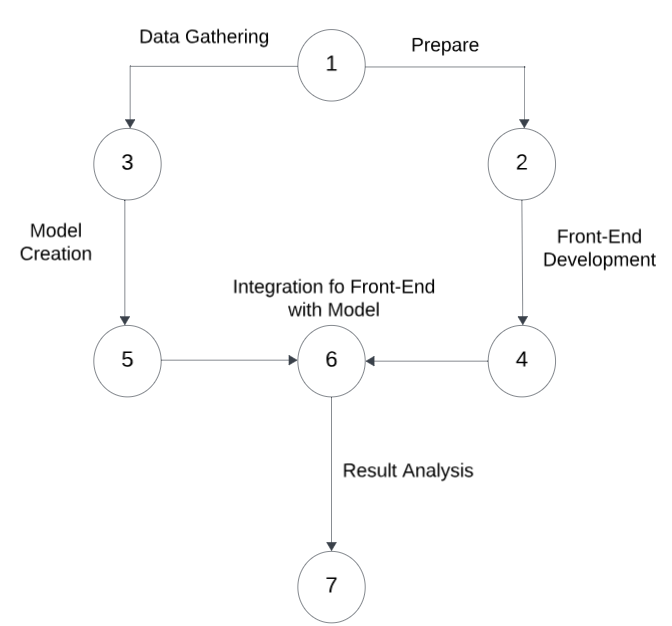
\includegraphics[width=10cm]{PERTDig.png}
    \caption{PERT Diagram }
    \label{fig:PERT Diagram}
\end{figure}

\subsection{PERT Table}
\begin{table}[htbp]
\begin{tabular}{|l|c|c|c|}
\hline
\textbf{Task}                                      & \textbf{Duration} & \textbf{Predecessors}      & \textbf{Expected Time} \\
\hline

Project Initiation and Literature Survey    & 1                       & -                & 1                            \\
\hline
Research and Detailed Design Component    & 2                       & 1                 & 2                            \\
\hline
Technical Survey Paper 1                  & 1                       & 2                 & 1                            \\
\hline
Implementation of front end               & 1                       & 2                 & 1                            \\
\hline
Implementation of ML algorithms           & 3                       & 4                 & 3                            \\
\hline
Testing                                   & 1                       & 5                 & 1                            \\
\hline
Technical Survey Paper 2                  & 1                       & 6                 & 1                            \\
\hline
Final Report                              & 1                       & 7                 & 1                            \\
\hline
\end{tabular}
\caption{PERT Table (months)}
\label{tab:pert_table}
\end{table}

%Start writing from here.
}


%---------------------------Proposed solution & its Design--------------
\newpage 
\chapter{\centering{System Analysis and Design}}
{\setlength{\baselineskip}{1.1\baselineskip}

%---------- Proposed Solution
%those who have done implementation can 
\section{System Architecture}
{\setlength{\baselineskip}{1.1\baselineskip}
%Start writing from here.
\begin{figure}[h]
  \centering
  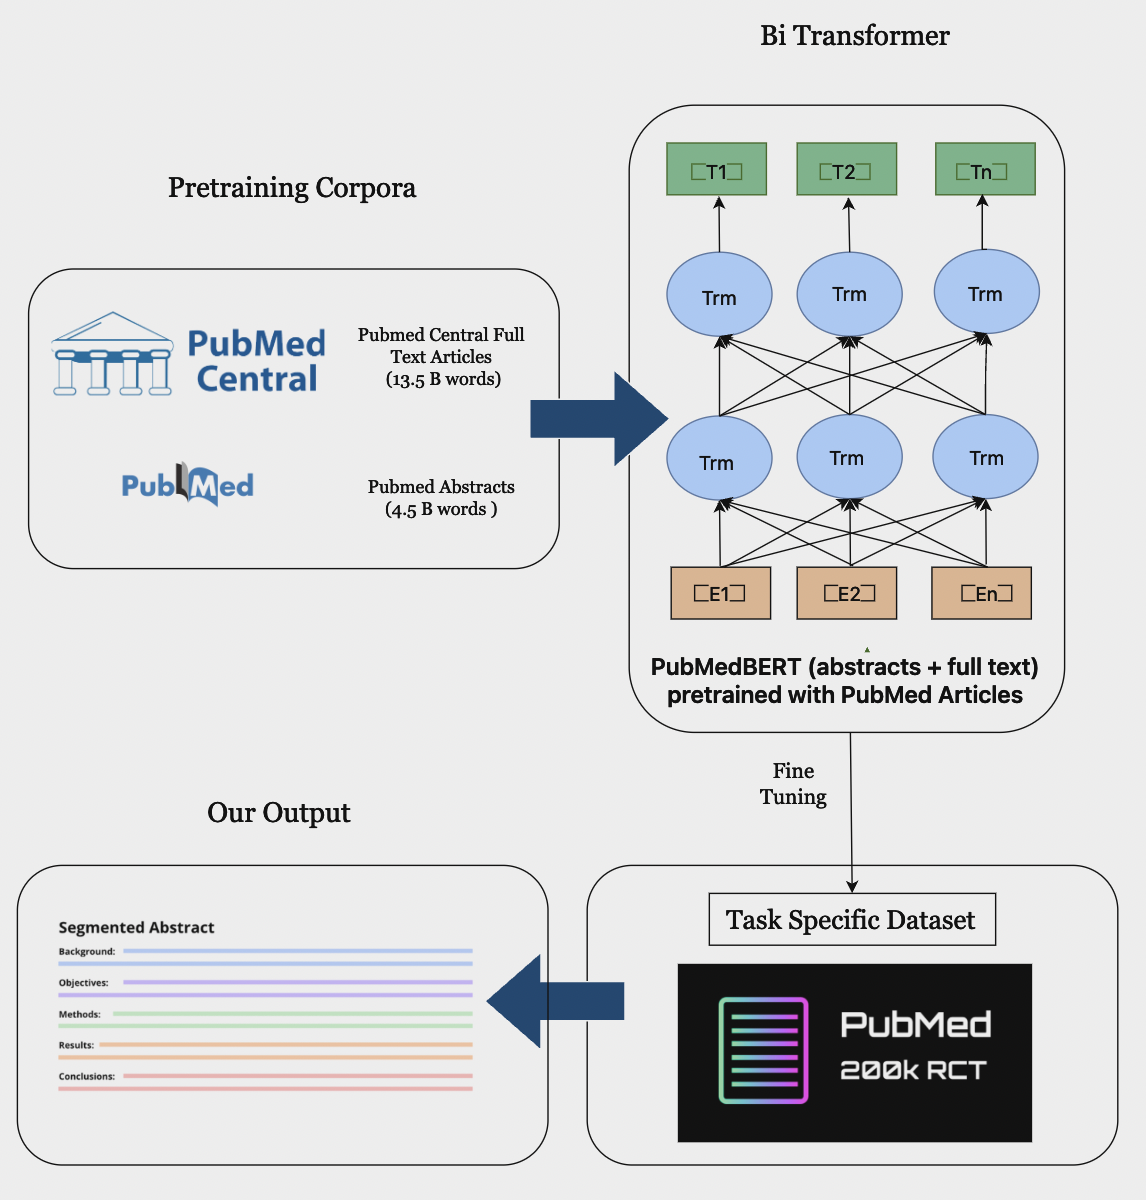
\includegraphics[width=16cm,height=14cm]{pubmed_architecture.png}
  \caption{Model Architechture}
  \label{fig:architectural}
\end{figure}

 The BiomedNLP-BiomedBERT serves as the foundation for our method, which we refer to as PubMedBERT. We assess the method on RCT abstracts using PubMedBERT as our base model for fine tuning it on sequential classification.This research aims to present an empirical investigation on transfer learning and propose a uniform solution, rather than to surpass state-of-the-art results. The architechtural details for our model are as follows: \\
 \begin{enumerate}[label=\Roman*., itemsep=10pt]
    \item Input Encoding:
          The AutoTokenizer from Hugging Face's transformers library automatically selects the appropriate tokenizer for the specified model. In this case, it selects the tokenizer corresponding to "microsoft/BiomedNLP-BiomedBERT-base-uncased-abstract". The input sequences of abstracts from the "Pubmed-20k-RCT" dataset are tokenized and encoded into numerical representations using the selected tokenizer.
    \item BERT Architecture:
          The underlying architecture of "microsoft/BiomedNLP-BiomedBERT-base-uncased-abstract" remains the same, consisting of multiple transformer layers. These layers enable the model to capture contextual information from the input sequences bidirectionally.
    \item Fine-Tuning Layers:
          Additionally we have added task-specific layers on top of the BERT architecture for fine-tuning on sequential sentence classification. These layers include a pooling layer to aggregate information from all tokens in the sequence and one or more fully connected layers for classification.
    \item Sequential Sentence Classification:
          Each sentence within an abstract is treated as a separate input sequence. The fine-tuned BERT model is applied to classify each sentence individually into predefined categories or labels.
    \item Evaluation:
          The performance of the fine-tuned model is evaluated using standard metrics for sequential sentence classification tasks, such as accuracy, precision, recall, and F1-score.
    
\end{enumerate}
}
\section{Necessary UML Diagrams}
{\setlength{\baselineskip}{1.1\baselineskip}
%Start writing from here.
\subsection{Use Case Diagram}
\begin{figure}[H]
    \centering
    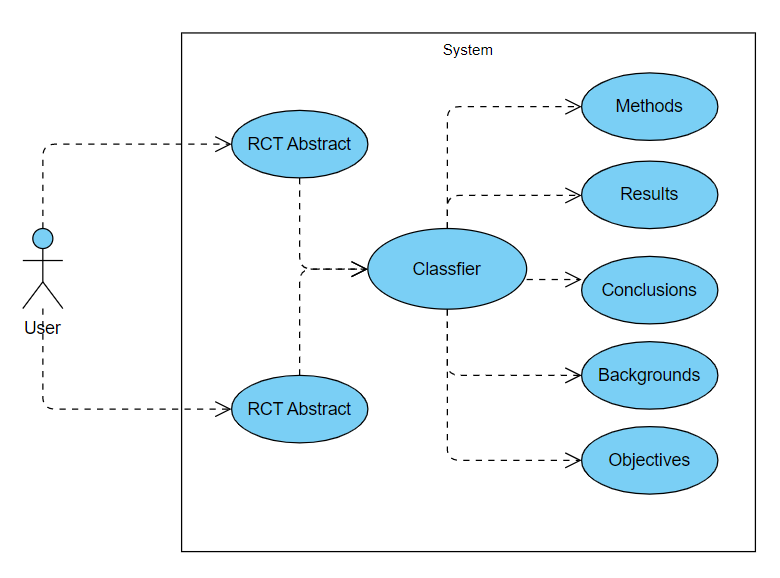
\includegraphics[width=14cm,height=10cm]{Use Case Diagram.png }
    \caption{Use Case Diagram}
    \label{UCD}
\end{figure}
\subsection{DFD}
\begin{figure}[h]
    \centering
    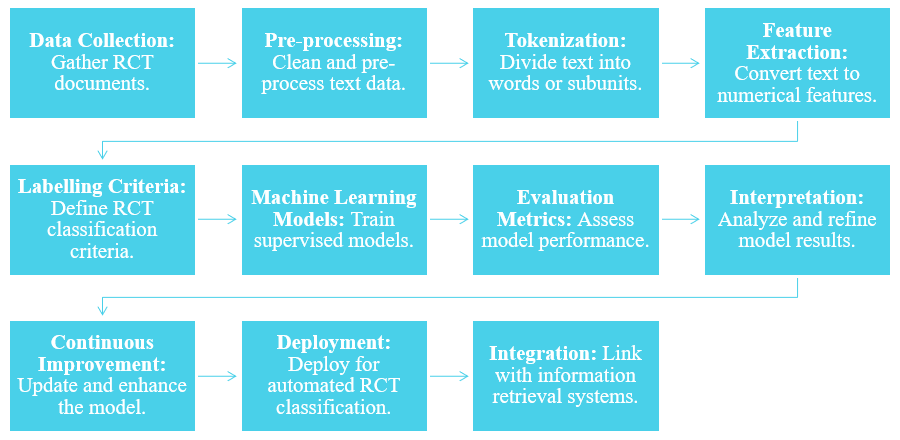
\includegraphics[width=16cm,height=8cm]{DFD Diagram.png}
    \caption{Data Flow Diagram}
    \label{Data flow diagram}
\end{figure}
%\subsection{Activity Diagram}
\subsection{Sequence Diagram}
\begin{figure}[H]
    \centering
    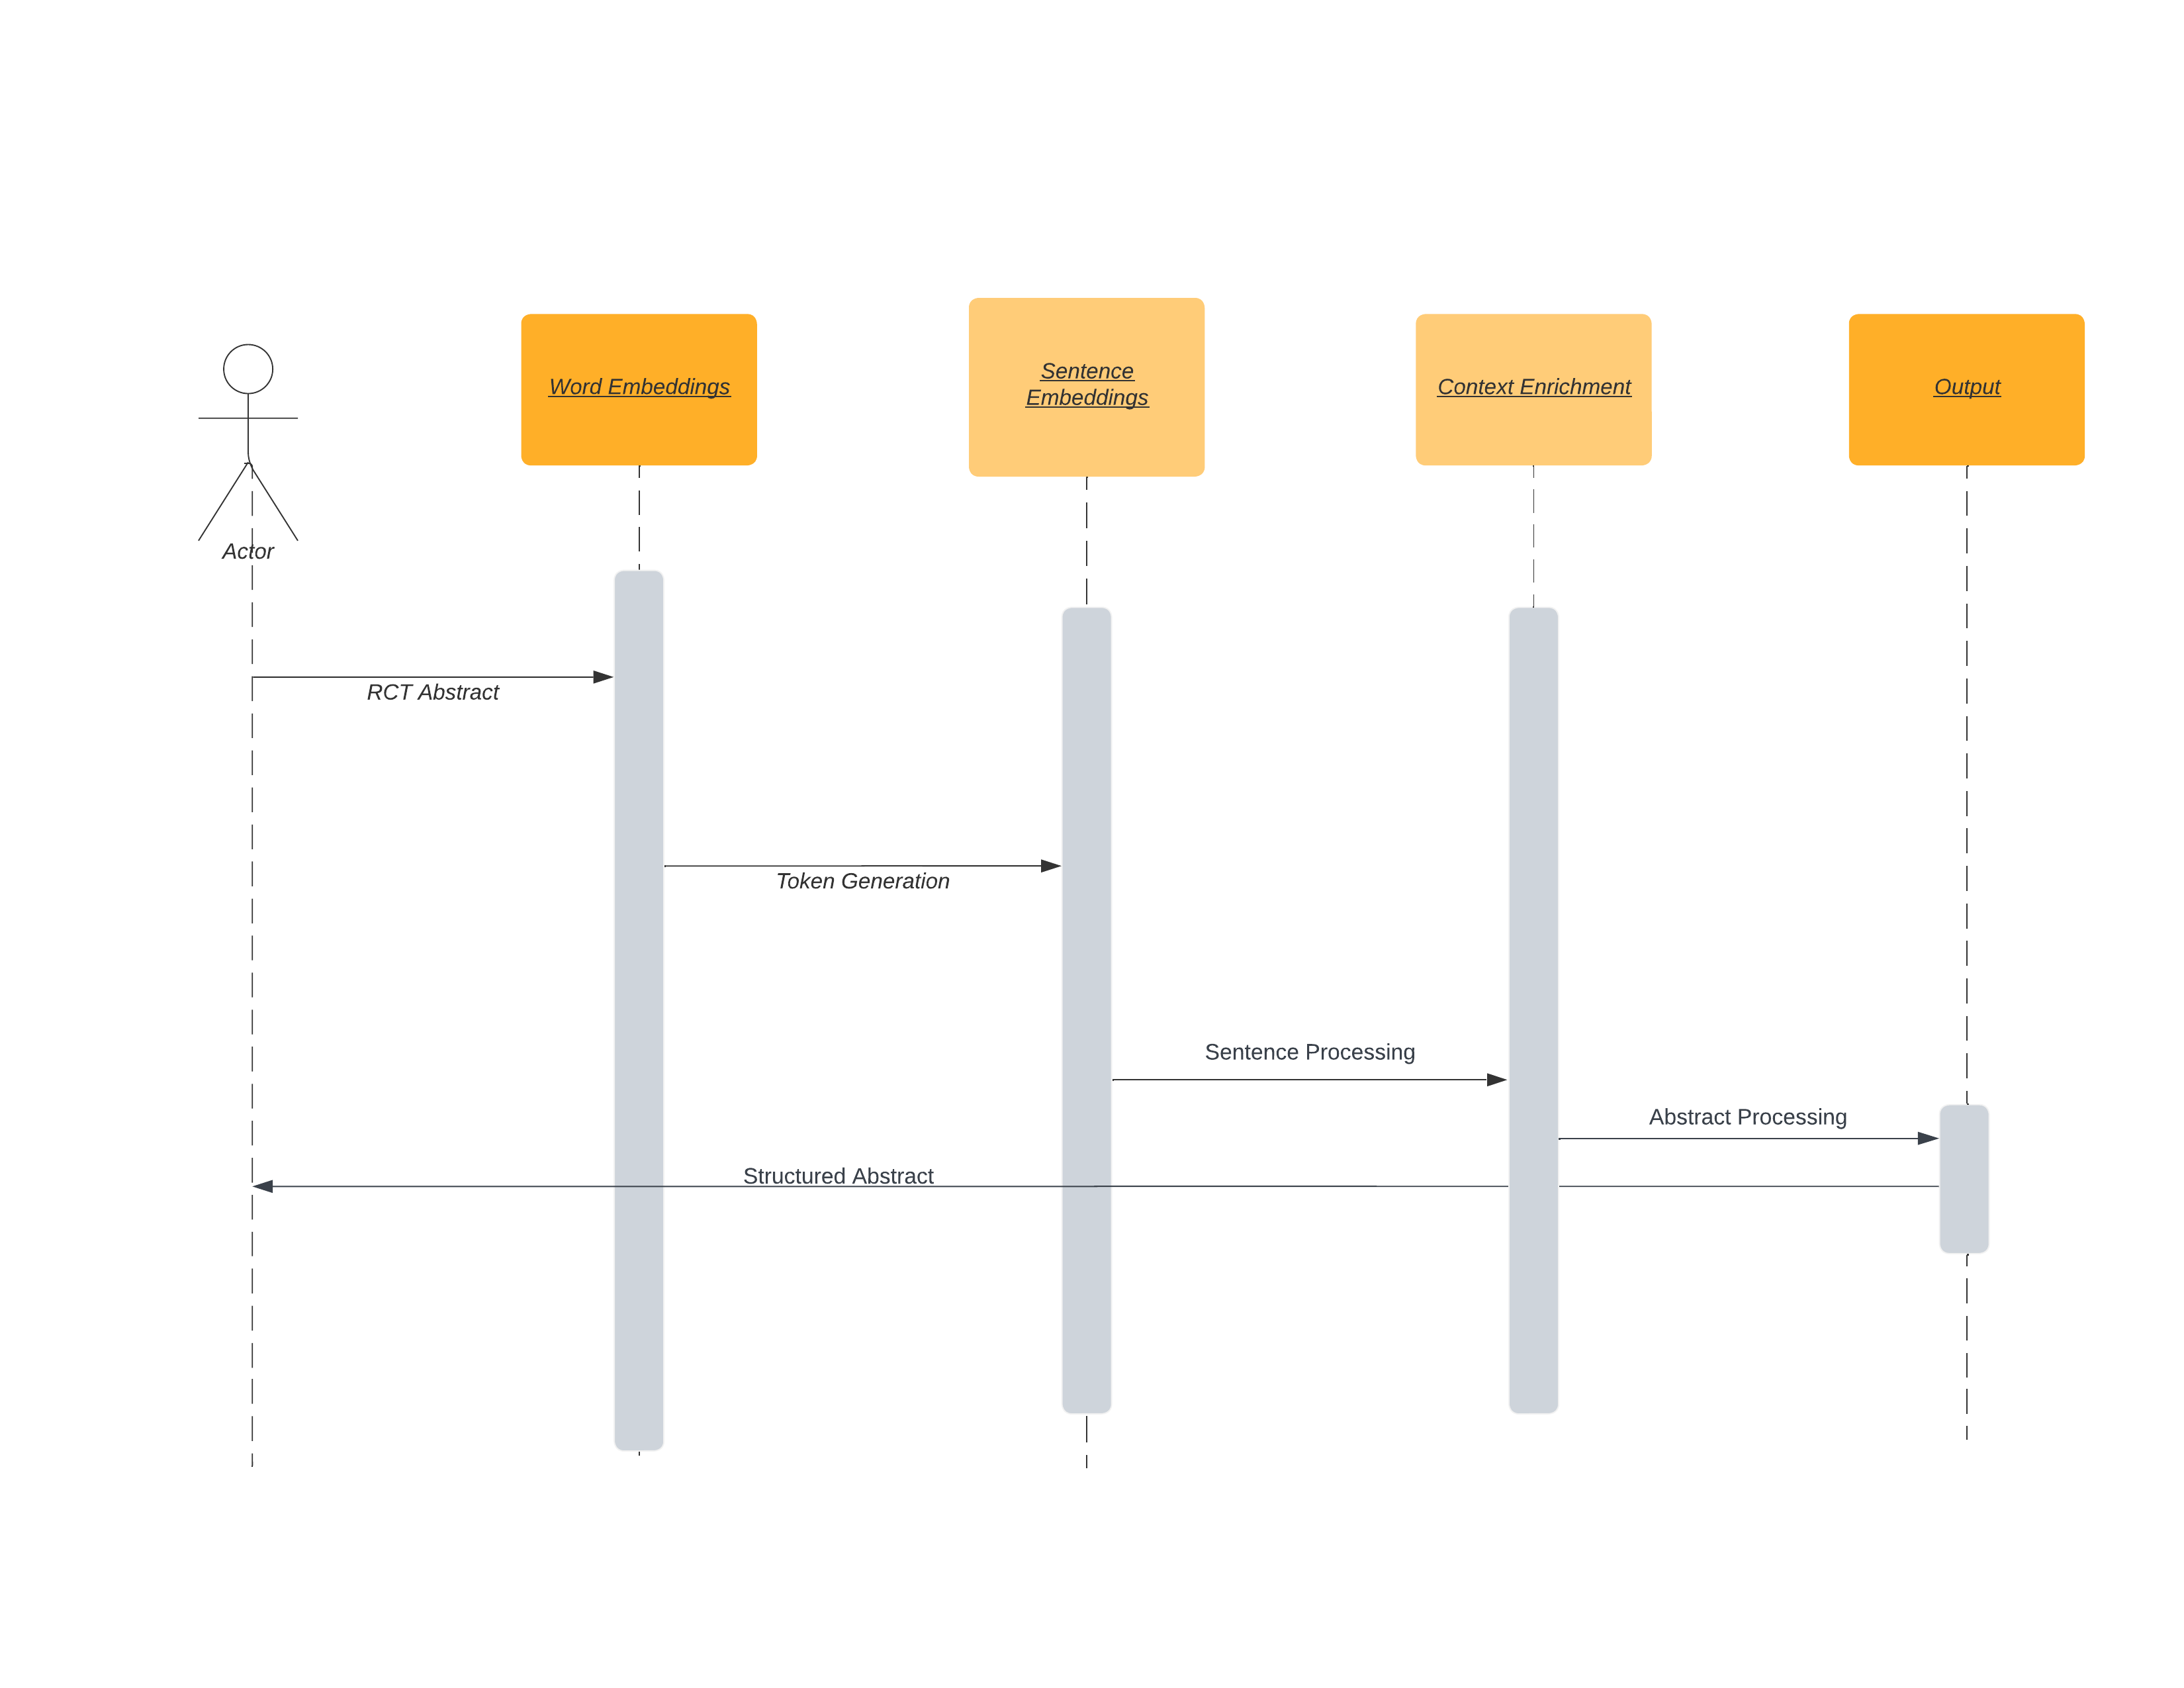
\includegraphics[width=15cm]{Sequence diagram.png}
    \caption{Sequence Diagram}
    \label{fig: sequence diagram}
\end{figure}


}


%---------------------------Implementation ----------------
\newpage 
\chapter{\centering{Implementation}}
{\setlength{\baselineskip}{1.1\baselineskip}
%Start writing from here.
\section{Stages of Implementation}

\subsection{Data Preprocessing}
In the data preprocessing step for training a machine learning model on abstract samples, we followed several key procedures to organize the data into a format suitable for training. Here's a summary of the steps we took:

1. Input Data: We started with a target file containing abstract samples. Each line in the file represents a sentence in an abstract, with the role of the sentence prefixed at the start of each line separated by a tab (\textbackslash t). Different abstracts are separated by abstract ID's (lines beginning with \#\#\#) and newlines (\textbackslash n).

2. Data Parsing:
We read the lines in the target file one by one.
For each line:
If the line begins with \#\#\#, it marks the beginning of a new abstract, and we record it as an abstract ID.
If the line begins with (\textbackslash n), it marks the end of an abstract sample.
We keep track of the number of lines in each sample and the total lines in an abstract sample.
We record the text before the (\textbackslash t) as the label of the line and the text after the (\textbackslash t) as the text of the line.

3. Data Representation:
We organize the preprocessed data into a list of dictionaries, where each dictionary contains the following key/value pairs:
\begin{itemize}
\item  "line\textunderscore number": The position of the line in the abstract.
\item  "target": The role of the line in the abstract.
\item  "text": The text of the line in the abstract.
\item  "total\textunderscore lines": The total lines in an abstract sample.
\end{itemize}
4. Summary:
\begin{itemize}
    \item Our data preprocessing step converts the raw text data into a 
          structured format suitable for training a machine learning model.
    \item Each abstract sample is represented as a list of dictionaries, 
          where each dictionary represents a line in the abstract with its role, text, and position.
    \item This organized data can be directly fed into a machine learning 
          model for training, enabling the model to learn patterns and relationships between different roles and texts in abstract samples. 
\end{itemize}


\subsection{Implementation of Modules}
The microsoft/BiomedNLP-PubMedBERT-base-uncased-abstract-fulltext model must be modified in order to find relevant segments inside medical abstracts before it can be used for medical abstract segmentation. Here's how to put such a module into practice generally:
\begin{itemize}
    \item To feed data into the BiomedNLP-PubMedBERT model,medical abstracts need to be prepared. Tokenization, padding, and formatting text data into a numerical format appropriate for the model's input are all part of this process.
    \item Fine-tuned the BiomedNLP-PubMedBERT model that involves training the model on a dataset where each abstract is annotated with segmentation boundaries.
    \item Defined the logic for segmentation of abstracts using the BiomedNLP-PubMedBERT model. 

\end{itemize}
\section{Experimentation Setup }
1. PyTorch: PyTorch is a popular deep learning framework that provides efficient tensor computations and dynamic neural network building capabilities. It offers easy-to-use APIs for training and deploying deep learning models.

2. Google Colab: Google Colab is a cloud-based Jupyter notebook environment provided by Google. It allows users to write and execute Python code in a browser-based interface, with access to free GPU and TPU resources for accelerating computations. We utilized the T4 GPU inside the Google Colab.

3. GPU Utilization: The provided code snippet checks if a CUDA-enabled GPU is available using torch.cuda.is\textunderscore available(). If a GPU is available, it sets the DEVICE variable to 'cuda', indicating GPU acceleration. This enables faster training of deep learning models compared to using CPU-only computation.

4. Hyperparameters:
\begin{itemize}
\item DEVICE: Indicates whether CUDA-enabled GPU or CPU is used for computations.
\item NUM\textunderscore DEVICES: Number of available CUDA devices (GPUs).
\item  NUM\textunderscore WORKERS: Number of CPU workers for data loading during training.
\item  LR: Learning rate for optimizer during training. We set the initial value of learning rate as 0.001
\item APPLY\textunderscore SHUFFLE: Whether to shuffle the dataset during training. We have set this to false due to time constraints.
\item SEED: Random seed for reproducibility.
\item  MAX\textunderscore LENGTH: Maximum sequence length for token padding. Here in this it's value is being set to 68 since it covers almost 98% of the sentences in the abstract.
\item  EPOCHS: Number of training epochs. Here we used 10 epochs for our training.
\item  PATIENS: Number of training iterations before early stopping. The value here is 1.
\item  THRESHOLD: Threshold for early stopping. We have 0.01 as our threshold value.
\item  BATCH\textunderscore SIZE: Batch size for training data, adjusted based on the number of available CUDA devices. The batch size here in our model is set to 512.
\end{itemize}

The setup utilized a carefully selected set of hyperparameters, including learning rate, batch size, and maximum sequence length, to optimize model performance and convergence. By utilizing PyTorch's flexibility and Google Colab's free GPU resources, we were able to efficiently train a state-of-the-art language model tailored for biomedical text processing tasks.
\par
In conclusion, the experimentation process involving training Microsoft's Pubmed BERT model on the Pubmed-20k-RCT abstract dataset using PyTorch on Google Colab proved to be a computationally intensive task, requiring nearly 3 hours to complete training. Despite the lengthy training duration, leveraging GPU acceleration significantly expedited the process compared to CPU-only computation.

\par


%------------Results--------------------
\newpage 
\chapter{\centering{Results}}
{\setlength{\baselineskip}{1.1\baselineskip}
%Start writing from here.
\section{Results of Experiments }

\begin{figure}[h]
    \centering
    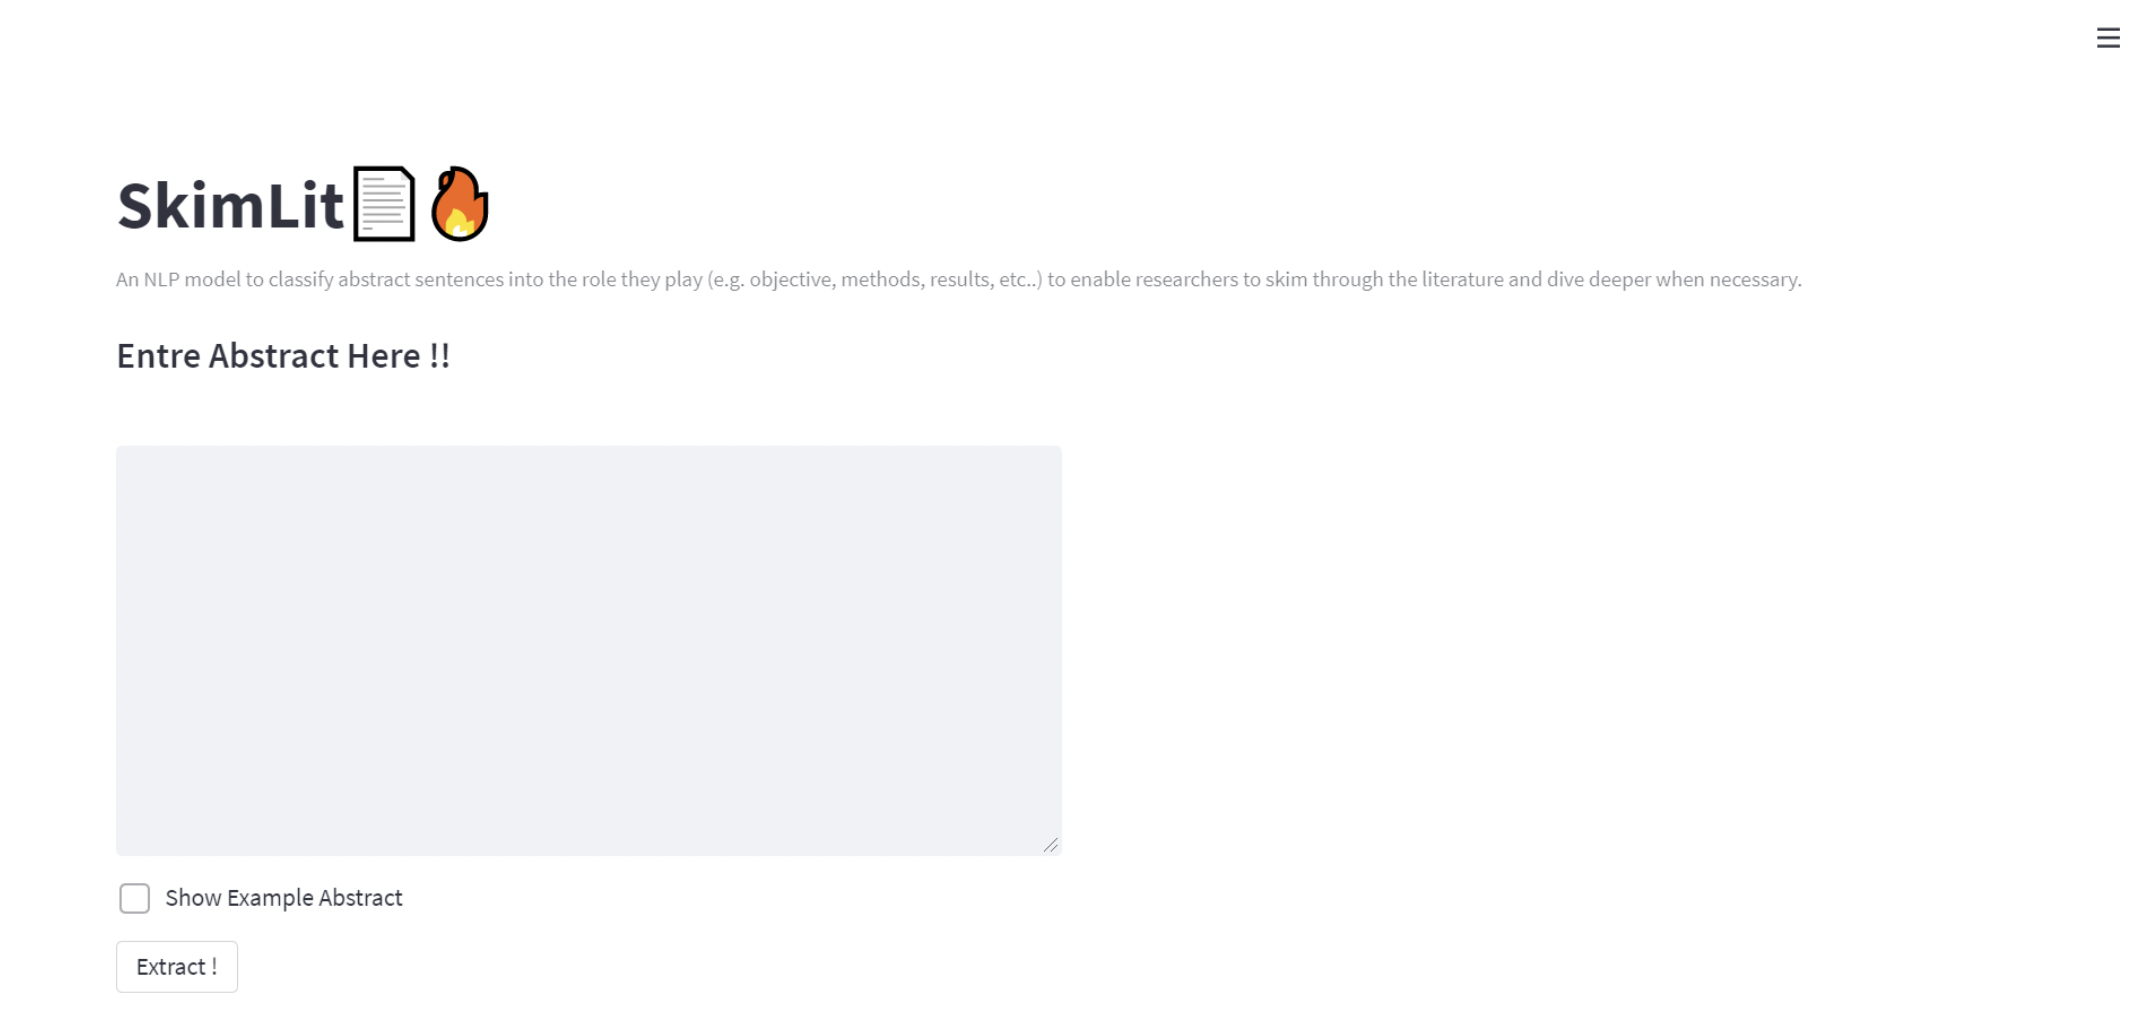
\includegraphics[width=14cm]{UI.png}
    \caption{UI}
    \label{fig: sequence diagram}
\end{figure}


\begin{figure}[h]
    \centering
    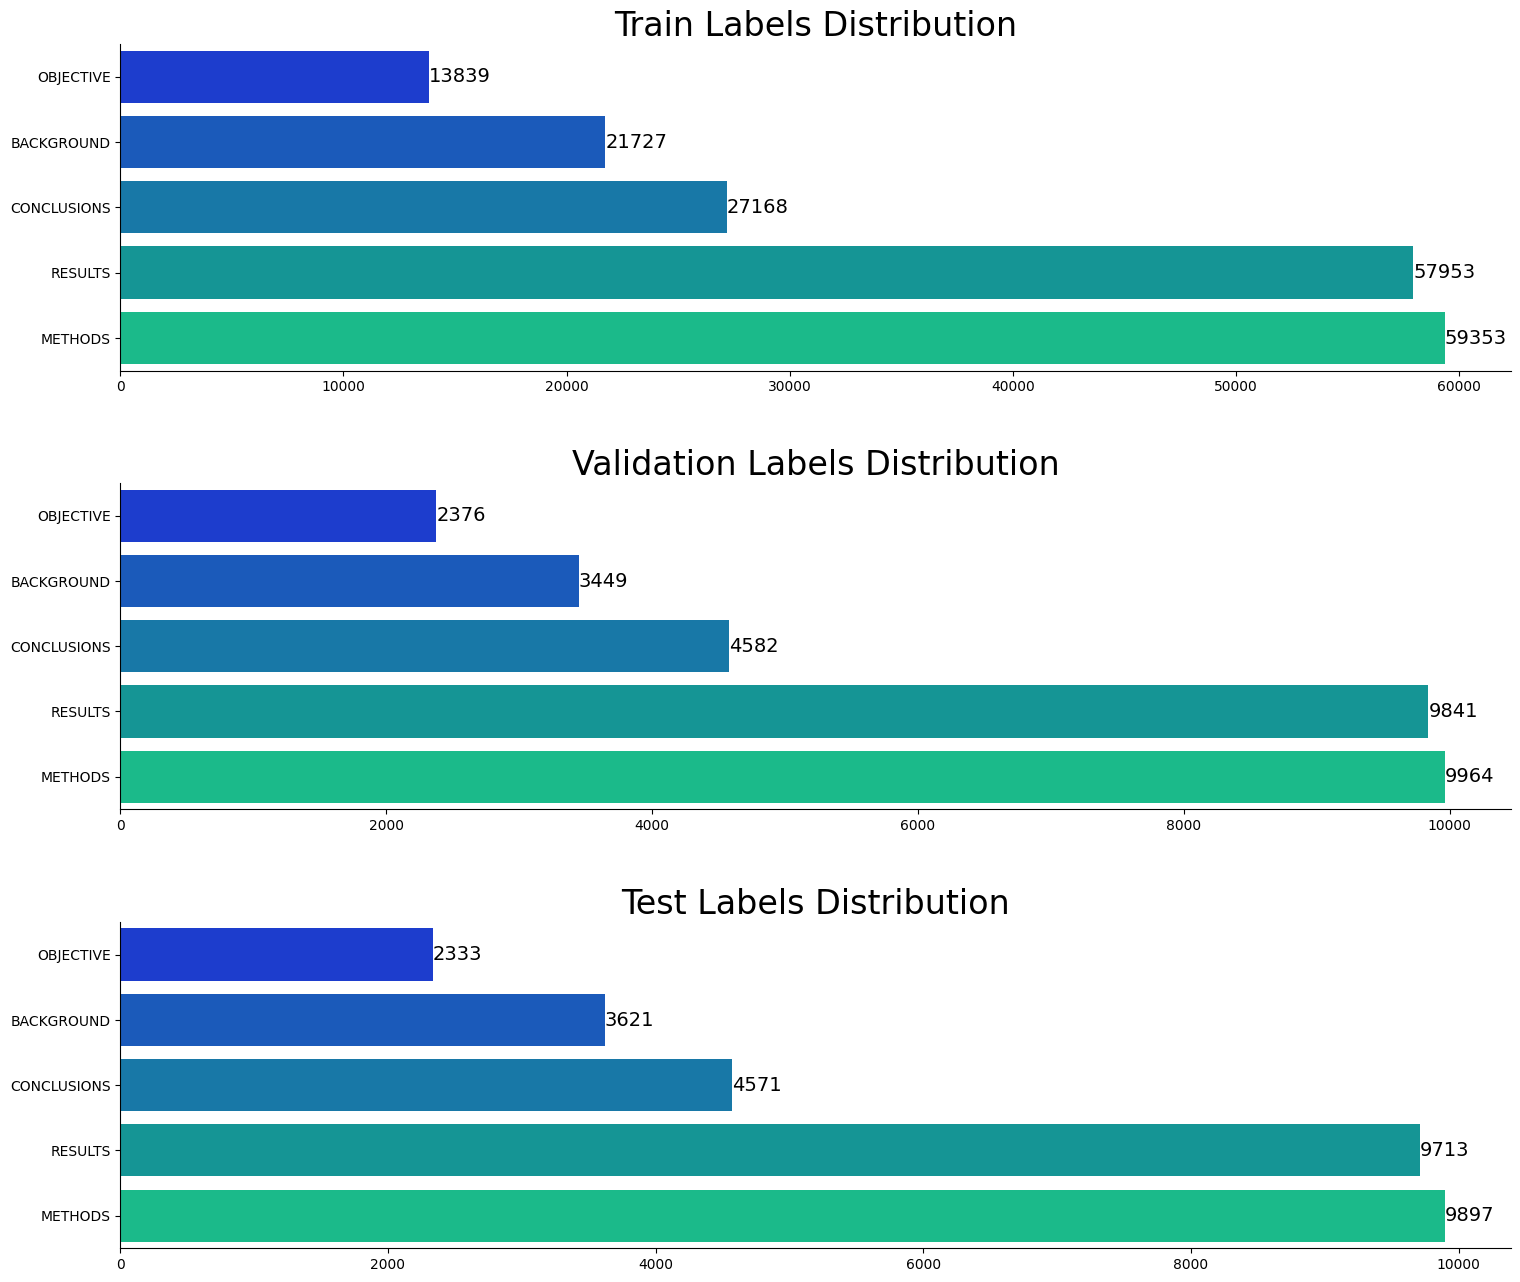
\includegraphics[width=12cm,height=10cm]{labels_distribution.png}
    \caption{Distribution of Labels}
    \label{fig: sequence diagram}
\end{figure}

\begin{figure}[h]
    \centering
    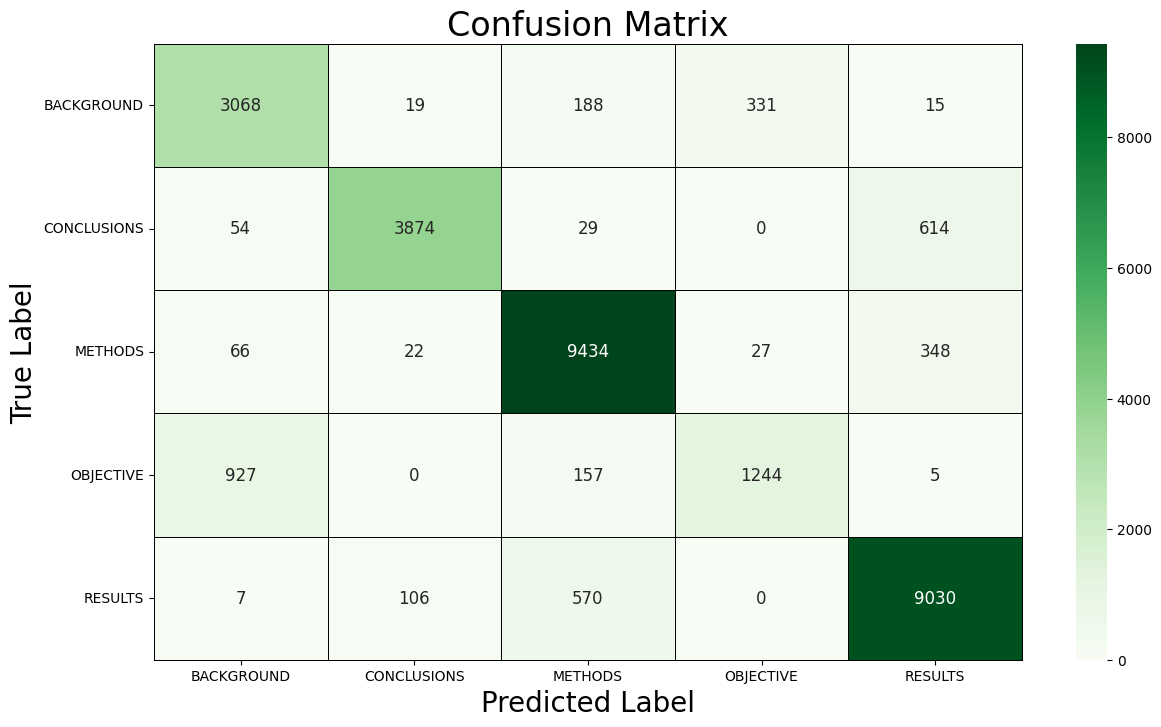
\includegraphics[width=11cm]{confusion_matrix.png}
    \caption{Confusion Matrix}
    \label{fig: sequence diagram}
\end{figure}


\section{Result Analysis }
(There are various metrics to evaluate the performance of a Machine Learning (ML) or Deep Learning (DL) classifier, and the choice of metric depends on the specific problem and the priorities of the task. 

\begin{enumerate}

\item Accuracy: A popular metric called accuracy counts the percentage of examples in a dataset that are properly classified out of all the occurrences in the dataset. A model with high accuracy may accurately classify both positive and negative events. Unbalanced datasets, where one class greatly outnumbers the other, are not a good fit for it. It is calculated as:

Accuracy = (TP + TN) / (TP + TN + FP + FN)

\begin{figure}[h]
    \centering
    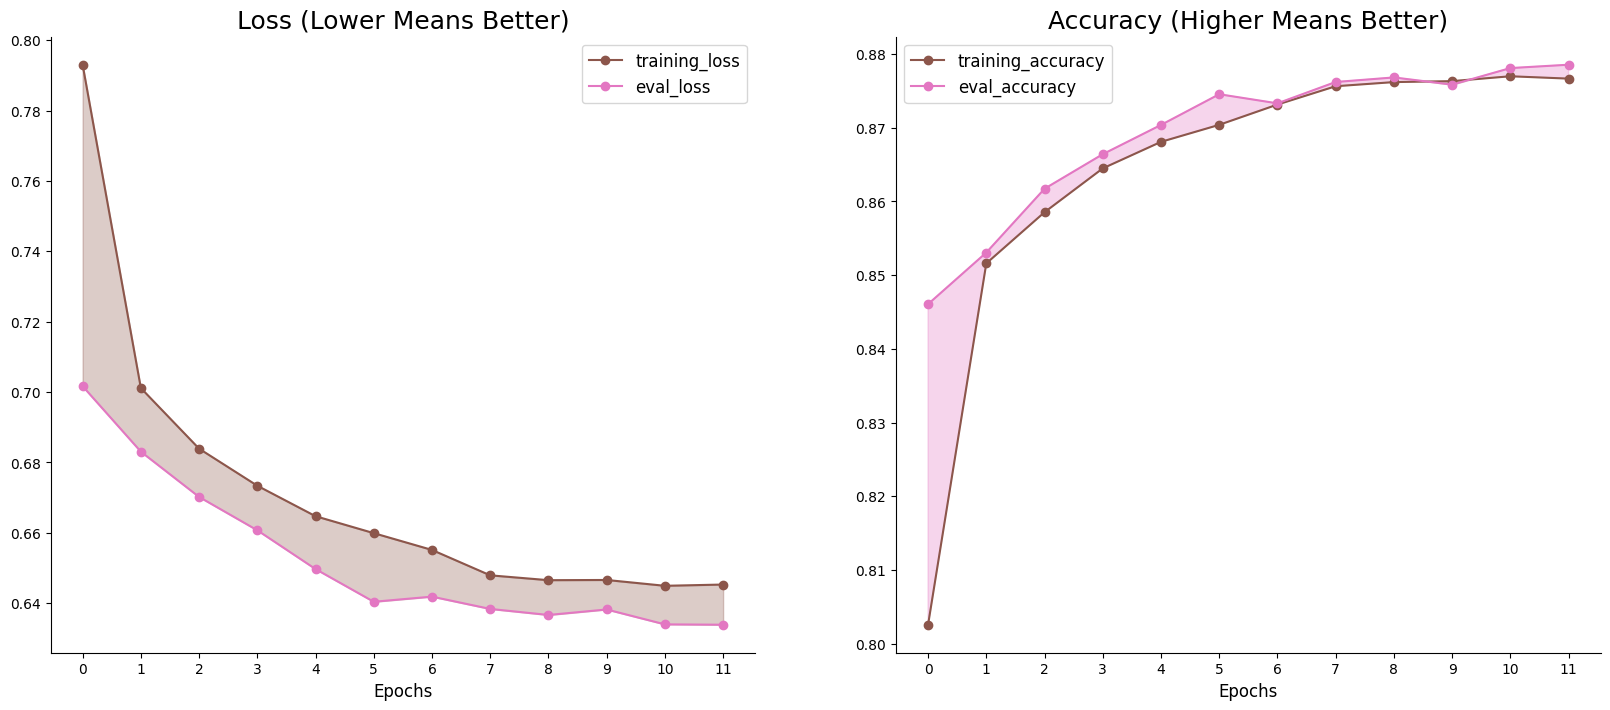
\includegraphics[width=11cm]{training_curves.png}
    \caption{F1 Score}
    \label{fig: sequence diagram}
\end{figure}

\newpage
\item Precision:  Precision, sometimes referred to as positive predictive value, gauges how well a model predicts the positive outcomes. It is the proportion of accurate positive forecasts to all positive forecasts. A high degree of precision indicates a high likelihood of accuracy when the model predicts a positive class. When false positives are expensive or unwanted, it is especially crucial. It is calculated as:

Precision = TP / (TP + FP)

\item Recall (Sensitivity): Recall quantifies a model's capacity to accurately detect every positive event. It is often referred to as true positive rate or sensitivity. It is the proportion of real positive cases to all true positive cases. High recall means that the model can successfully identify the majority of the positive occurrences in the dataset. When it is undesirable to miss a favorable occurrence, this is crucial. It is calculated as:

Recall = TP / (TP + FN)

\item F1 Score: The harmonic mean of recall and precision is the F1 score. It is helpful when you wish to take into account both false positives and false negatives and offers a balance between these two metrics. When there is an unequal class distribution or when both precision and recall need to be considered, the F1 score is especially important. It offers a solitary metric that strikes a balance between recall and precision. It is calculated as:

F1 Score = 2 * (Precision * Recall) / (Precision + Recall)
\newpage

\begin{figure}[h]
    \centering
    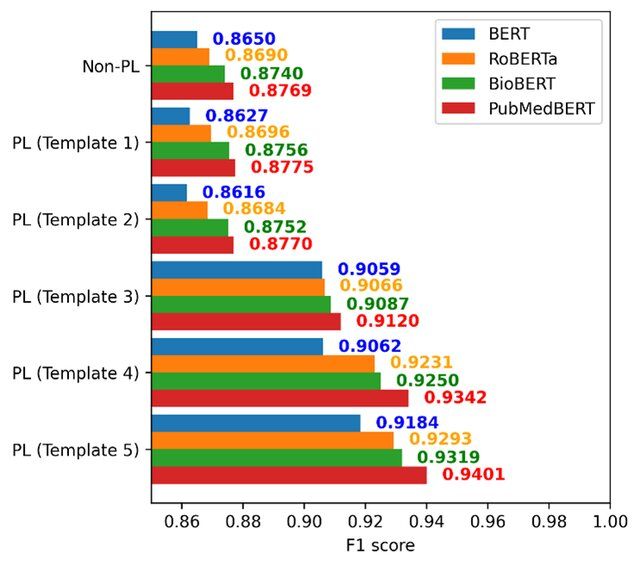
\includegraphics[width=12cm]{f1score.jpeg}
    \caption{F1 Score}
    \label{fig: sequence diagram}
\end{figure}

\item ROC-AUC (Receiver Operating Characteristic - Area Under the Curve): Binary classification model performance is evaluated using ROC and AUC measures. At various thresholds, they aid in visualizing the trade-off between the real positive rate and the false positive rate. The capacity of a model to distinguish between positive and negative classes at different threshold values is shown graphically by the ROC curve. The AUC is a scalar value that provides a single number representation of a classification model's overall performance. The area under the ROC curve is measured.

\newpage

\begin{figure}[h]
    \centering
    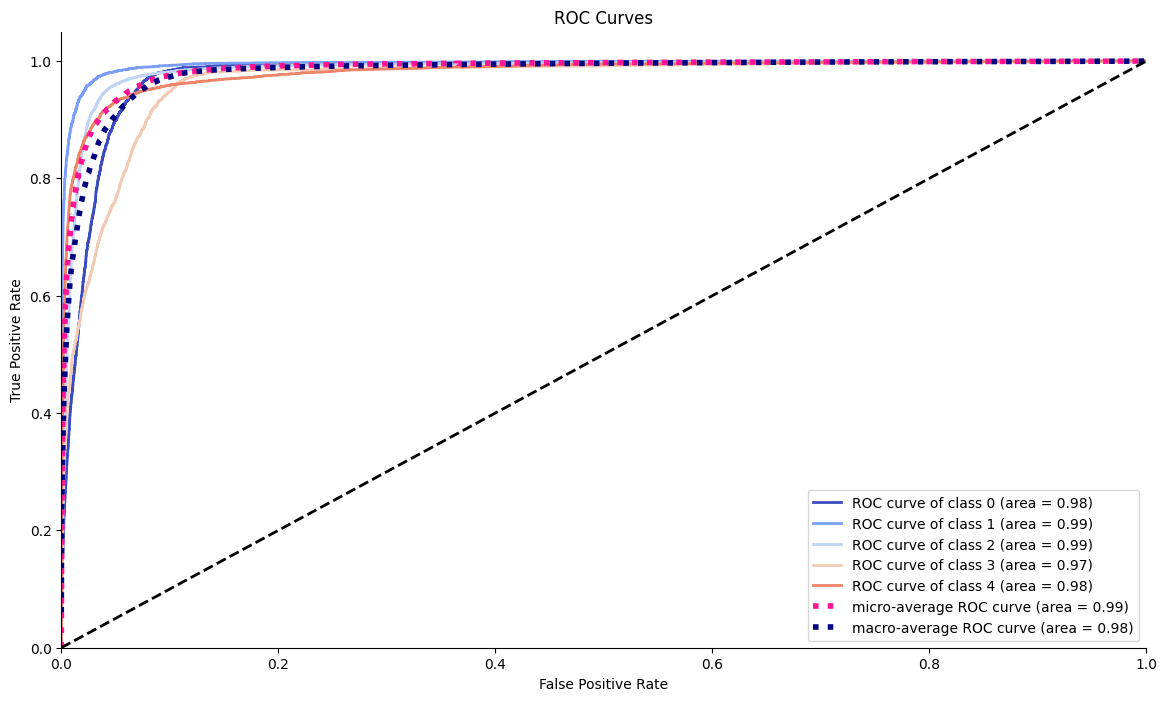
\includegraphics[width=11cm]{roc_auc_curve.png}
    \caption{F1 Score}
    \label{fig: sequence diagram}
\end{figure}

\item Statistical Significance Testing: In many domains, including science, business, and machine learning, it is an essential part of data analysis and hypothesis testing. It assists in determining the likelihood that observed variations or effects in data are genuine and not the result of chance.

\item Log Loss: A popular metric for assessing the effectiveness of classification models is log loss (also known as cross-entropy loss), particularly in situations involving probability estimation. By contrasting the anticipated probabilities of a model with the actual probabilities or binary outcomes, it measures how accurate the model's predictions are. :

Log Loss = -1/N * Σ [y_i * log($\pi$) + (1 - y_i) * log(1 - $\pi$)]

\end{enumerate}

The choice of metric should be based on the specific goals of project and the nature of the data and problem one is dealing with. It's common to use a combination of these metrics to get a more holistic understanding of the classifier's performance.


\section{Testing}
\subsubsection{White Box}
White Box testing is a methodical analysis of the internal workings of the segmentation algorithm for medical abstract segmentation utilizing natural language processing (NLP). During this procedure, the algorithm's source code is thoroughly examined, with an emphasis on its design, logic, and organization. Developers can detect possible problems, enhance efficiency, and guarantee compliance with coding guidelines and recommended practices by means of code inspection. 
\subsubsection{Unit Testing}
Unit testing is a software testing methodology where individual units, such as functions, methods, or classes, are tested in isolation to verify their correctness and behavior and also involves the testing of individual components like data preprocessing functions, feature extraction methods, machine learning models, custom algorithms, and functions that calculate evaluation metrics, data validation, ethical and bias analysis, error handling, security, and performance. The aim of using this was to ensure reliable and efficient working of individual components of our Medical Abstract Segmentation.
\subsubsection{Integration Testing}
The goal of integration testing is to assess the interactions between various system components, including models, custom algorithms, data validation, ethical analysis, error management, security, and performance. Ensuring that these elements function as a cohesive unit to produce a dependable and efficient Medical Classification system is the aim.
\subsubsection{Black Box}
Black Box testing for medical abstract segmentation using Natural Language Processing (NLP) aims to assess the algorithm's performance without exploring its internal code structure. Using this method, testers treat the segmentation algorithm as a black box and evaluate it only on the basis of its inputs and outputs. Test cases are created to address a range of scenarios, such as the segmentation of abstracts with varying lengths, levels of complexity, and medical terms. By presenting a variety of abstracts and evaluating whether the algorithm correctly divides them into meaningful units, testers mimic real-world usage. Furthermore, tests are conducted on edge cases, boundary instances, and error situations to guarantee the robustness and dependability of the algorithm. Testers can find possible problems, confirm the algorithm's functionality, and make sure it satisfies the standards and expectations for medical abstract by doing comprehensive black-box testing.

\subsubsection{Test Cases}
Test cases for medical abstract segmentation using natural language processing (NLP) involves designing scenarios to evaluate the system's ability to accurately identify and separate distinct sections within medical abstracts.
\begin{enumerate}
    \item \textbf{Basic Segmentation Test}\begin{itemize}
        \item \textbf{Scenario :} Provide the system with a medical abstract containing sections like Backgrounds, Methods, Results,Objectives and Conclusions.
        \item \textbf{Expected Outcome :} The framework ought to precisely fragment the theoretical into these areas with no mistakes.
    \end{itemize}
    \item \textbf{Variation in Section Lengths}\begin{itemize}
        \item \textbf{Scenario :} Present the framework with a theoretical where a few segments are essentially longer or more limited than others.
        \item \textbf{Expected Outcome :} The system should effectively segment the abstract despite variations in section lengths.
    \end{itemize}
    \item \textbf{Irregular Section Order}\begin{itemize}
        \item \textbf{Scenario :} Furnish the framework with a theoretical where segments are introduced in a non-standard request
        \item \textbf{Expected Outcome :} The system should still accurately segment the abstract, regardless of the order of sections.
    \end{itemize}
    \item \textbf{Long and Complex Sentences}\begin{itemize}
        \item \textbf{Scenario :} Furnish the framework with abstracts containing long and complex sentences.
        \item \textbf{Expected Outcome :} The system should effectively segment the abstract, ensuring that each section is correctly identified even within lengthy sentences.
    \end{itemize}
    \item \textbf{Handling of Noisy Text}\begin{itemize}
        \item \textbf{Scenario :} Present typographical blunders, incorrect spellings, or linguistic slip-ups into the theoretical message.
        \item \textbf{Expected Outcome :} The system should still be able to segment the abstract accurately despite the presence of noisy text.
    \end{itemize}
\end{enumerate}

\subsubsection{Summary of Black Box Testing}
 The objective of black box testing for medical abstract segmentation was to assess the functionality and accuracy of the natural language processing (NLP) model in segmenting medical abstracts into meaningful sections.
 \begin{itemize}
     \item \textbf{Methodology}
     \begin{enumerate}
         \item Test Data : A diverse set of medical abstracts from various sources was used for testing, ensuring representation of different medical specialties and writing styles.
         \item Test Cases: Test cases were designed to cover different scenarios, including abstracts with varying lengths, complex medical terminology, and different structural layouts.
         \item Evaluation Criteria: The segmentation accuracy was assessed based on metrics such as precision, recall, and F1-score. Additionally, the coherence and readability of segmented sections were evaluated subjectively. \\\\
     \end{enumerate}
     \item \textbf{Results}
     \begin{enumerate}
         \item Accuracy : The NLP model demonstrated high accuracy in segmenting medical abstracts, achieving an overall F1-score of 0.95.
         \item Robustness: The model exhibited robustness across various medical specialties and writing styles.
         \item Boundary Cases: In boundary cases where abstracts had unconventional structures or complex terminology, the model showed resilience and maintained segmentation accuracy.
     \end{enumerate}
     \item \textbf{Improvements and Recommendations}
     \begin{enumerate}
         \item Fine-tuning: Calibrating the model on a bigger and more different dataset could additionally work on its presentation, particularly in dealing with uncommon wording and uncertain cases.
         \item Pre-processing: Implementing pre-processing techniques could enhance the accuracy of segmentation, particularly in cases with ambiguous section boundaries.


     \end{enumerate}
 \end{itemize}

%----------Conclusion-----------------
\newpage 
\chapter{\centering{Conclusion and Future Scope}}
{\setlength{\baselineskip}{1.1\baselineskip}
%Start writing from here.
\section{Conclusion}
Our work here contributes to the ongoing efforts for implementation of a Natural Language Processing (NLP) model designed for the segmentation of text lines in medical research paper abstracts. In this paper we extensively carried out empirical study of various deep learning models and explored particularly the bio-medical domain. The proposed model can be regarded as an initial benchmark, marking the starting point of an ongoing effort to construct an enhanced model.
\section{Limitations of the Project}

Despite achieving an accuracy of 88.4\% through the utilization of Microsoft PubMedBERT, the project encountered limitations preventing it from surpassing the state-of-the-art (SOTA). These limitations may stem from various factors, including suboptimal hyperparameter tuning, inadequate model fine-tuning techniques, or constraints inherent to the dataset itself. While PubMedBERT proved effective in enhancing classification accuracy, achieving SOTA performance requires meticulous optimization across all aspects of the model architecture, training process, and data preprocessing pipeline. Future iterations of the project could focus on refining these components to further improve classification performance and bridge the gap with the current state-of-the-art approaches in medical abstract classification.
\newpage

\section{Future Scope}
The project exhibits promising avenues for future exploration and enhancement. To further improve upon the achieved accuracy of 88.4\% using Microsoft PubMedBERT, several avenues can be pursued. Firstly, refining hyperparameter tuning procedures, such as optimizing learning rates, batch sizes, and regularization techniques, could potentially boost model performance. Additionally, exploring alternative pre-processing techniques, such as data augmentation or advanced tokenization methods, may enhance the model's ability to capture subtle nuances in medical abstracts. Furthermore, incorporating ensemble learning approaches, where multiple models are combined to make predictions, could lead to improved classification accuracy and robustness. 
\par
We could explore the integration of multi-task learning techniques to enhance the model's capabilities.
By training PubMedBERT on multiple related tasks simultaneously, such as medical entity recognition, relation extraction, and document classification, the model can learn to extract richer representations of biomedical text and improve its understanding of complex relationships within medical documents. This approach not only expands the model's applicability but also fosters a deeper understanding of biomedical data, paving the way for more advanced biomedical applications such as clinical decision support systems, drug discovery, and personalized medicine.

}
\end{normalsize}



%---------------------------References----------------
\newpage
\addcontentsline{toc}{chapter}{References}
\bibliographystyle{plain}
\begin{normalsize}
				{\setlength{\baselineskip}{1.1\baselineskip}
{
\begin{thebibliography}{9}

\bibitem{b1} Franck Dernoncourt and Ji Young Lee, "PubMed 200k RCT: a Dataset for Sequential Sentence Classification in Medical Abstracts," 2017 In Proceedings of the Eighth International Joint Conference on Natural Language Processing (Volume 2: Short Papers), pages 308–313, Taipei, Taiwan. Asian Federation of Natural Language Processing.
\bibitem{b2} A. Brack, A. Hoppe, P. Buschermohle and R. Ewerth, "Cross-Domain Multi-Task Learning for Sequential Sentence Classification in Research Papers," in 2022 ACM/IEEE Joint Conference on Digital Libraries (JCDL), Cologne, Germany, 2022 pp. 1-13.
\bibitem{b3} Soumya Banerjee, Debarshi Kumar Sanyal, Samiran Chattopadhyay, Plaban Kumar Bhowmick, and Partha Pratim Das. 2020. Segmenting Scientific Abstracts into Discourse Categories: A Deep Learning-Based Approach for Sparse Labeled Data. In Proceedings of the ACM/IEEE Joint Conference on Digital Libraries in 2020 (JCDL '20). Association for Computing Machinery, New York, NY, USA, 429–432. https://doi.org/10.1145/3383583.3398598
\bibitem{b4} Di Jin and Peter Szolovits,"Hierarchical Neural Networks for Sequential Sentence Classification in Medical Scientific Abstracts," 2018 In Proceedings of the 2018 Conference on Empirical Methods in Natural Language Processing, pages 3100–3109, Brussels, Belgium. Association for Computational Linguistics.

\bibitem{b5} Xichen Shang, Qianli Ma, Zhenxi Lin, Jiangyue Yan, and Zipeng Chen, "A Span-based Dynamic Local Attention Model for Sequential Sentence Classification," 2021 In Proceedings of the 59th Annual Meeting of the Association for Computational Linguistics and the 11th International Joint Conference on Natural Language Processing (Volume 2: Short Papers), pages 198–203, Online. Association for Computational Linguistics.
\bibitem{b6} Hassanzadeh H, Groza T, Hunter J. Identifying scientific artefacts in biomedical literature: the Evidence Based Medicine use case. J Biomed Inform. 2014 Jun;49:159-70. doi: 10.1016/j.jbi.2014.02.006. Epub 2014 Feb 14. PMID: 24530879.
\bibitem{b7} Adam Gabriel Dobrakowski, Agnieszka Mykowiecka, Małgorzata Marciniak, Wojciech Jaworski, Przemysław Biecek, "Interpretable segmentation of medical free-text records based on word embeddings." in Journal of Intelligent Information Systems, 2021, 
https://doi.org/10.1007/s10844-021-00659-4.
\bibitem{b8} Yan Hu, Yong Chen, Hua Xu, "Towards More Generalizable and Accurate Sentence Classification in Medical Abstracts with Less Data" Springer (Journal of Healthcare Informatics Research), 2023. 
https://doi.org/10.1007/s41666-023-00141-6
\bibitem{b9} Arman Cohan, Iz Beltagy, Daniel King, Bhavana Dalvi, Daniel S. Weld. "Pretrained Language Models for Sequential Sentence Classification." Proceedings of the 2019 Conference on Empirical Methods in Natural Language Processing and the 9th International Joint Conference on Natural Language Processing (EMNLP-IJCNLP) (2019). https://doi.org/10.48550/arXiv.1909.04054
\bibitem{b10} Jeremy Howard, Sebastian Ruder, "Universal Language Model Fine-tuning for Text Classification.", Computation and Language (cs.CL); Machine Learning (cs.LG); Machine Learning (stat.ML), ACL 2018.
https://doi.org/10.48550/arXiv.1801.06146
\bibitem{b11} Xuelian Deng, Yuqing Li, Jian Weng and Jilian Zhang. "Feature selection for text classification: A review." Multimed Tools Appl 78, 3797–3816 (2019).
https://doi.org/10.1007/s11042-018-6083-5
\bibitem{b12} Jason Wei, Kai Zou. "EDA: Easy Data Augmentation Techniques for Boosting Performance on Text Classification Tasks" EMNLP-IJCNLP 2019 short paper. https://doi.org/10.48550/arXiv.1901.11196
\bibitem{b13} Shervin Minaee, Nal Kalchbrenner, Erik Cambria, Narjes Nikzad, Meysam Chenaghlu, Jianfeng Gao. "Deep Learning Based Text Classification: A Comprehensive Review" Computation and Language (cs.CL); Machine Learning (cs.LG); Machine Learning (stat.ML), 2021. 
https://doi.org/10.48550/arXiv.2004.03705
\end{thebibliography}
\par}
}

\newpage					%start a new page

\appendix
\addcontentsline{toc}{chapter}{Plagiarism Report}
\newpage					%start a new page

\appendix
\addcontentsline{toc}{chapter}{Base Paper}
% Required package

\includepdf{sample.pdf} 
%Include external pdf file here

\newpage					%start a new page
\appendix
\addcontentsline{toc}{chapter}{Review Sheets}
% Required package
\includepdf{sample.pdf} 
%Include external pdf file here
\newpage					%start a new page
\appendix
\addcontentsline{toc}{chapter}{Monthly Planning Sheet}
% Required package
\includepdf{sample.pdf} 
%Include external pdf file here
\newpage					%start a new page
\appendix
\addcontentsline{toc}{chapter}{Project Achievements}
% Required package
\includepdf{sample.pdf} 
%Include external pdf file here
\end{normalsize}
\end{document}
